\documentclass[
	% -- opções da classe memoir --
	12pt,				% tamanho da fonte
	openright,			% capítulos começam em pág ímpar (insere página vazia caso preciso)
	oneside,			% para impressão em verso e anverso. Oposto a oneside
	a4paper,			% tamanho do papel. 
	% -- opções da classe abntex2 --
	%chapter=TITLE,		% títulos de capítulos convertidos em letras maiúsculas
	%section=TITLE,		% títulos de seções convertidos em letras maiúsculas
	%subsection=TITLE,	% títulos de subseções convertidos em letras maiúsculas
	%subsubsection=TITLE,% títulos de subsubseções convertidos em letras maiúsculas
	% -- opções do pacote babel --
	english,			% idioma adicional para hifenização
	french,				% idioma adicional para hifenização
	spanish,			% idioma adicional para hifenização
	brazil				% o último idioma é o principal do documento
	dvipsnames, table]{abntex2}
\usepackage{graphicx} % Required for inserting images
\usepackage{xcolor}
\usepackage{longtable}
% \usepackage{subfigure}
\usepackage{float}
\usepackage{subfig}
\usepackage{url}


\title{4_resultados_rascunho}
\author{Matheus Ferreira de Souza}
\date{July 2024}

\begin{document}

\maketitle

\newpage

\chapter{Apresentação dos Resultados}

\section{Análise e discussão dos resultados}

\indent Como forma de otimizar a leitura, os resultados serão apresentados e discutidos na sequência. Também como facilitação, a ordem e numeração apresentados seguirão os mesmos adotados na metodologia. Para analisar de forma mais detalhada, os resultados se encontram no \href{https://github.com/matheusf30/dengue/tree/main/resultados}{GitHub}, publicados no endereço eletrônico abaixo:\\
\url{https://github.com/matheusf30/dengue/tree/main/resultados}\\


\section{Análise Estatística Descritiva \textcolor{red}{Climatologia}}

\indent Para melhor compreensão da descrição climatológica, acompanhe a tabela \textcolor{red}{(ou quadro?)} (tabela \ref{tab:valores_climato}) abaixo:

\begin{table}[htbp]
    \centering
    \caption{Valores estaduais de variáveis climatológicas}
    {\rowcolors{1}{lightgray}{white}
    \begin{tabular}{r|cccc}
    \hline
    \toprule
    \rowcolor{darkgray} \textcolor{white}{Valores Estaduais} & \textcolor{white}{Mínima} & \textcolor{white}{Média} & \textcolor{white}{Máxima} & \textcolor{white}{Desvio Padrão}\\
    \midrule
    Temperatura Mínima Diária & -7,98 C & 14,75 C& 30,26 C & 4,88 C\\
    Temperatura Mínima Semanal & -2,77 C & 14,75 C & 26,15 C & 4,11 C\\
    Temperatura Média Diária & -4,39 C & 18,66 C & 36,14 C & 4,78 C\\
    Temperatura Média Semanal & 1,68 C & 18,66 C & 33,67 C & 4,19 C\\
    Temperatura Máxima Diária & -1,21 C & 24,31 C & 40,72 C & 5,41 C\\
    Temperatura Máxima Semanal & 7,94 C & 24,31 C & 37,91 C & 4,52 C\\ 
    Precipitação Diária & 0,0 mm & 4,3 mm & 261,25 mm & 12,68 mm\\
    Precipitação Semanal & 0,0 mm & 30,07 mm & 478,25 mm & 43,05 mm\\
    \bottomrule
    \end{tabular}}
    \label{tab:valores_climato}
\end{table}

\indent Sobre a temperatura mínima diária, o menor valor que a série histórica do Estado de \acrlong{SC} apresentou foi de -7,98 C, sendo -2,77 C quando agrupado semanalmente. O valor máximo da temperatura mínima foi de 30,26 C, dados diários, e 26,15 C, dados semanais. A média diária da temperatura mínima para o Estado foi de 14,75 C, sendo o mesmo valor quando agrupado em semana, e o maior desvio padrão de 4,88 C para dados diários. O desvio padrão semanal foi de 4,11 C.

\indent Em se tratando de temperatura média diária, o menor valor que a série histórica do Estado de \acrlong{SC} apresentou foi de -4,39 C, sendo 1,68 C para dados semanais. O valor máximo da temperatura média foi de 36,14 C, dados diários, e 36,14 C, dados semanais. A média diária da temperatura mínima para o Estado foi de 18,66 C, tanto para valores diários quanto semanais, e o desvio padrão foi de 4,78 C e 4,19 C, dados diários e semanais, respectivamente. 

\indent Para a temperatura máxima diária, o menor valor foi de -1,39 C, sendo 7,94 C para dados semanais. O valor máximo da temperatura máxima foi de 40,72 C, dados diários, e 37,91 C, dados semanais. A média diária da temperatura máxima para o Estado de \acrlong{SC} foi de 24,31 C, tanto para valores diários quanto semanais, e o desvio padrão foi de 5,41 C e 4,52 C, dados diários e semanais, respectivamente.

\indent Todas as temperaturas apresentaram comportamento semelhante, mínima, média e máxima, por compartilharem o mesmo método de agrupamento semanal, baseado na média dos dias da semana. Logo, tem-se valores de máximas e mínimas próximos a média quando agrupados semanalmente e os valores de médias diárias e semanais são semelhantes, por conta do próprio método. Essa suavização por agrupamento também é verificada no desvio padrão, sendo menor em dados semanais. 

\indent A precipitação na série histórica de \acrlong{SC} obteve seu maior valor em 261,25 mm diários e 478,25 mm semanais. O menor valor foi zero (0) mm e igual em ambos os períodos analisados, diários ou semanais. A média de precipitação para o Estado é de 4,3 mm diários e 30,07 mm semanais, tendo 12,68 mm e 43,05 mm como desvio padrão para dados diários e semanais, respectivamente.

\indent O comportamento da precipitação é menos suave aos dados agrupados semanalmente, diferente das temperaturas. Porém, assim como as temperaturas, esse comportamento é por conta do método de agrupamento, baseado no somatório dos dias da semana. Logo, os valores semanais de precipitação são maiores, sejam eles médio, máximo ou desvio padrão. O valor mínimo diário e semanal é semelhante, zero (0) mm, pois há períodos em que não precipita em \acrlong{SC} por mais de sete (7) dias. Esse valor também diz respeito a característica do dado, sendo uma variável quantitativa de razão, em contraposição às temperaturas, que são variáveis quantitativas intervalares.

\indent \textcolor{red}{Interessante Amplitude Térmica? (Debater com o Mário)\\
Como aplicar Amplitude a esses dados?}

\section{Modelagem Preditiva}

\subsection{Pré-processamento}

\indent Durante o processo de estruturação de dados, todos os 295 municípios catarinenses apresentaram valores para todas as variáveis climatológicas em questão (precipitação e temperaturas mínima, média e máxima). Esse fato foi possível por adotarmos o valor do centróide do polígono atual do município para extração dos dados, assim, municípios recentes apresentam valores climatológicos mesmo antes de sua emancipação, como Pescaria Brava. Uma nota deve ser tomada, pois o valor do centróide do polígono do município não coincide com o ponto central urbano da cidade.

\indent Em contraposição, o mesmo não ocorre com as variáveis epidemiológicas e entomológicas. Os \acrshort{DEE} apresentam poucos registros municipais no início das séries históricas disponíveis, além de serem mais recentes. Como exemplo, 2017 foi o ano com apenas cinco (5) municípios registrando casos de dengue dentro do Estado catarinense, sendo eles: Brusque, Guaraciaba, Itajaí, Itapema e Sombrio. Por isso a padronização das datas de todas as séries históricas, que foi assumido valor zero (0) para o período antes do primeiro registro de cada município. Dessa mesma maneira, tem-se o primeiro registro de cada município, para a séries históricas catarinenses tanto de focos de \latim{Aedes} sp. (tabela \ref{tab:primeiros_focos}) quanto de casos de dengue (tabela \ref{tab:primeiros_casos}), ambas as tabelas disponibilizadas em Apêndices.



% \begin{figure}[htbp]
%     \centering
%     \caption{Mapa evidenciando o recorte espacial dos dados relacionados à região sul do brasil. Visualização dos dados de temperatura mínima durante o solstício de inverno de 2023.}
%     \includegraphics[scale=0.5]{climatologia_tmin_2023-06-21.pdf}
%     \label{fig: sul_brasil}
%     \\
%     \vspace{-0.05cm}\hspace{-7.5cm}\small{Fonte: Elaboração própria (2024).} 
% \end{figure}


\subsection{Processamento}

% Realizadas entre os \acrshort{DEE} (focos de \latim{Aedes} sp. e casos de dengue)
\indent As quatro (4) cidades elencadas nos estudos foram: Florianópolis, Itajaí, Joinville e Chapecó; por apresentarem frequência e volume de dados, além de representarem regiões populosas e distintas. Sobre as correlações, realizadas pelo método de \textcolor{red}{Spearman}, o máximo de retroação foi em 16 semanas epidemiológicas entre focos de \latim{Aedes} sp. e casos de dengue. Foram analisados os anos de 2020, 2021, 2022 e 2023, assim como a própria série histórica, porém apenas será apresentado o ano de 2023 (figura \ref{fig: matriz_corr_DEE}).

\begin{figure}[htbp]
    \centering
    \caption{Matriz de correlações entre focos de \latim{Aedes} sp. e casos de dengue de alguns municípios catarinenses durante 2023, método de Spearman.}
    \label{fig: matriz_corr_DEE}
    \subfloat[Florianópolis \label{fig: corr_DEE_FLO}]{
        \centering
        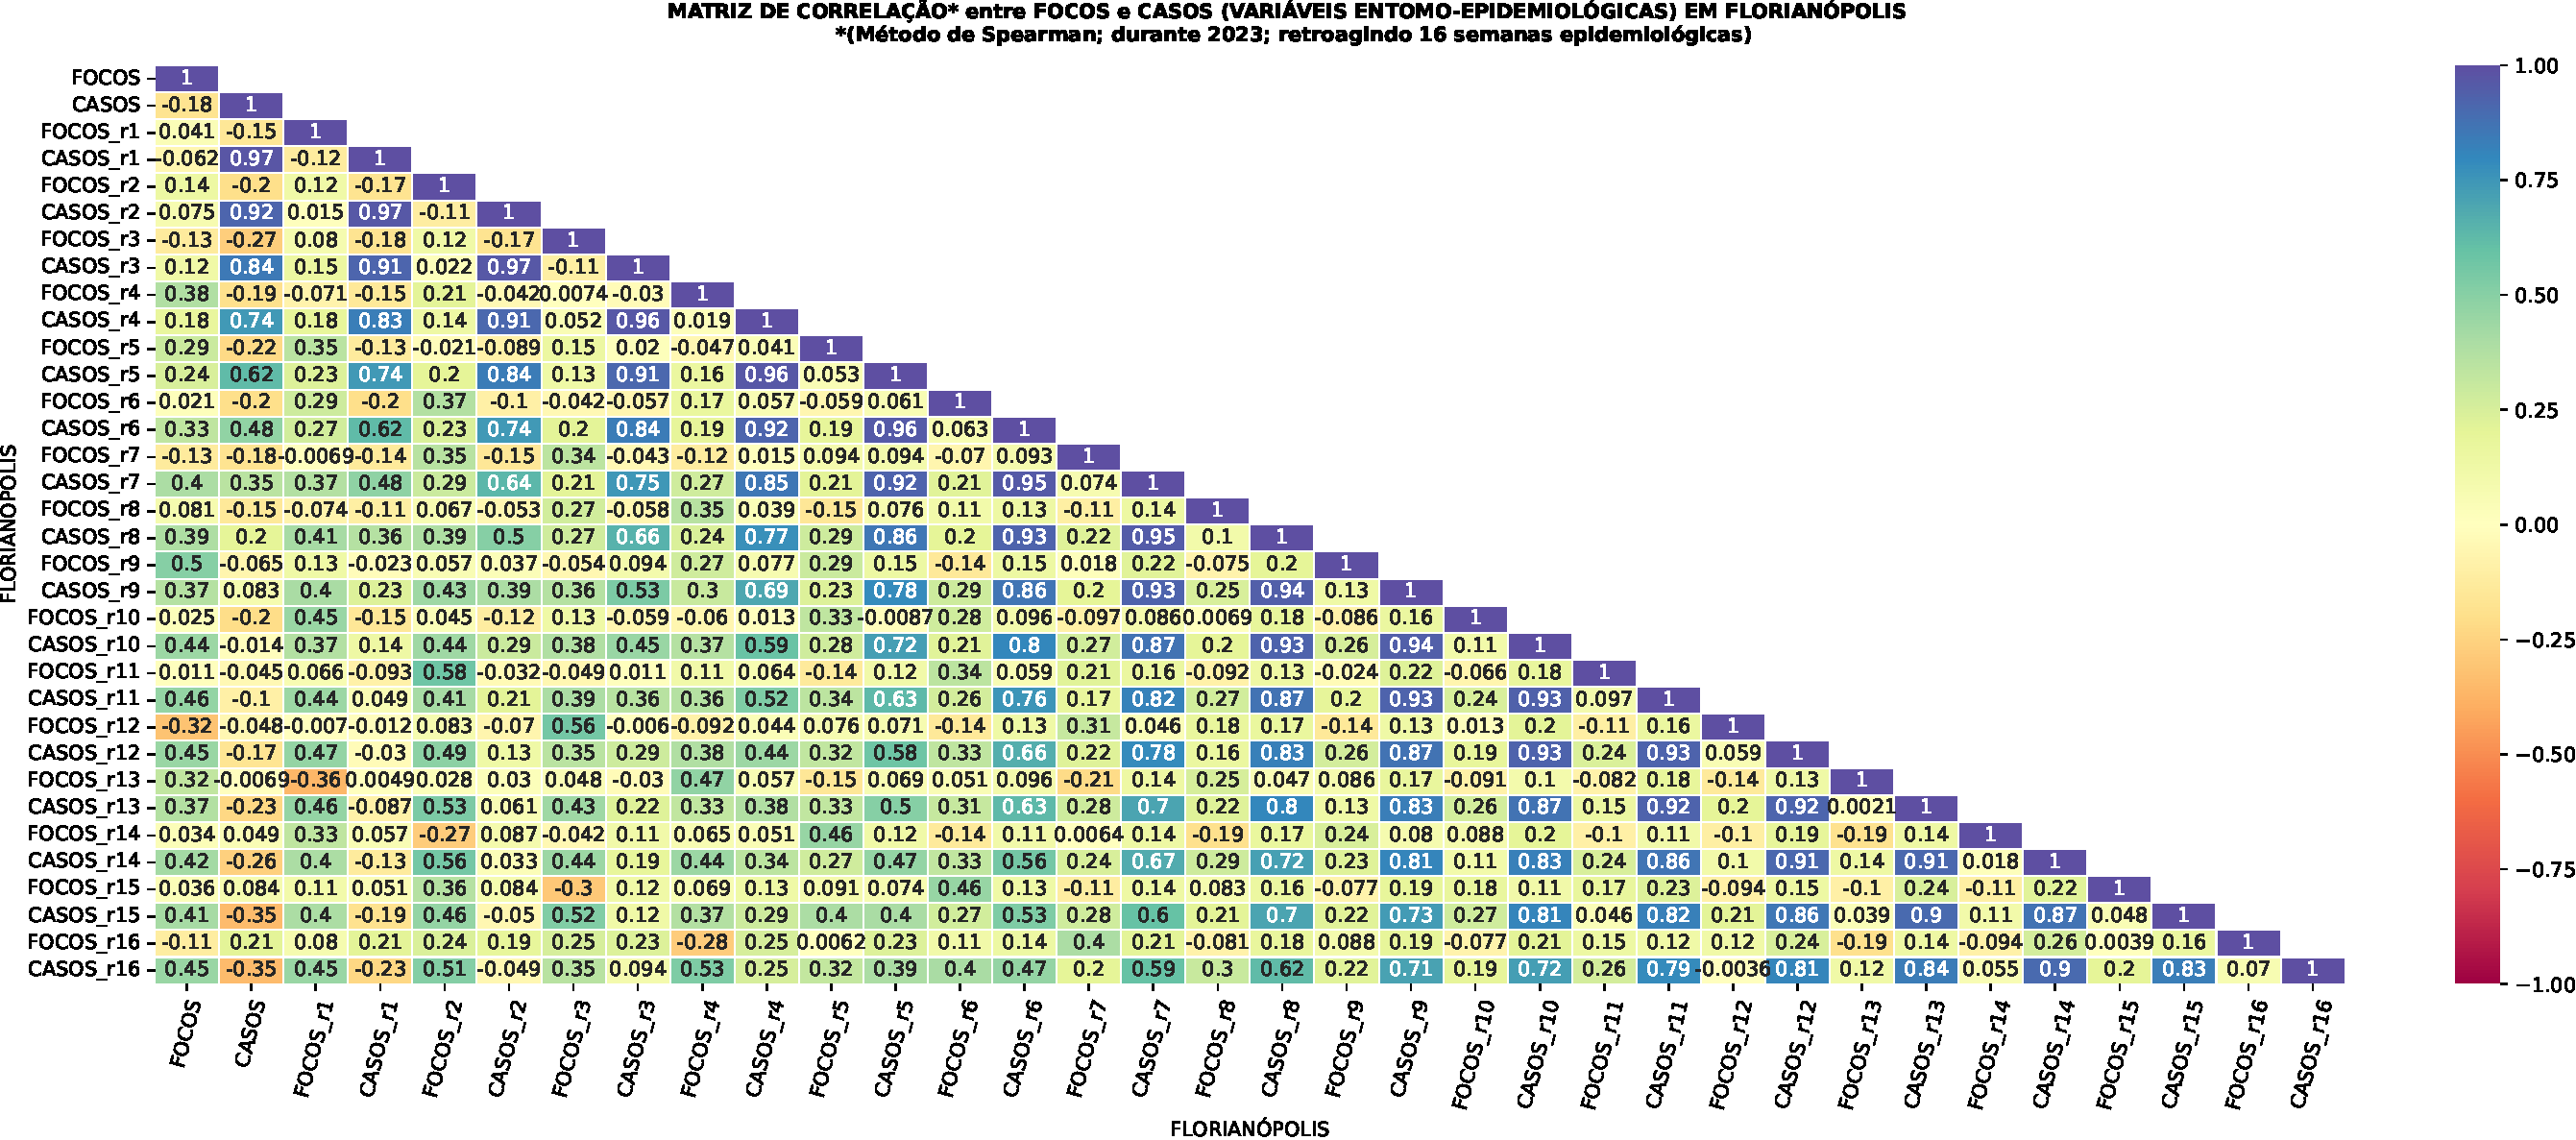
\includegraphics[width=0.47\textwidth]{figuras/matriz_correlacao_spearman_fococaso_FLORIANOPOLIS_r16s_2023.pdf}
        }
    \subfloat[Itajaí \label{fig: corr_DEE_ITA}]{
        \centering
        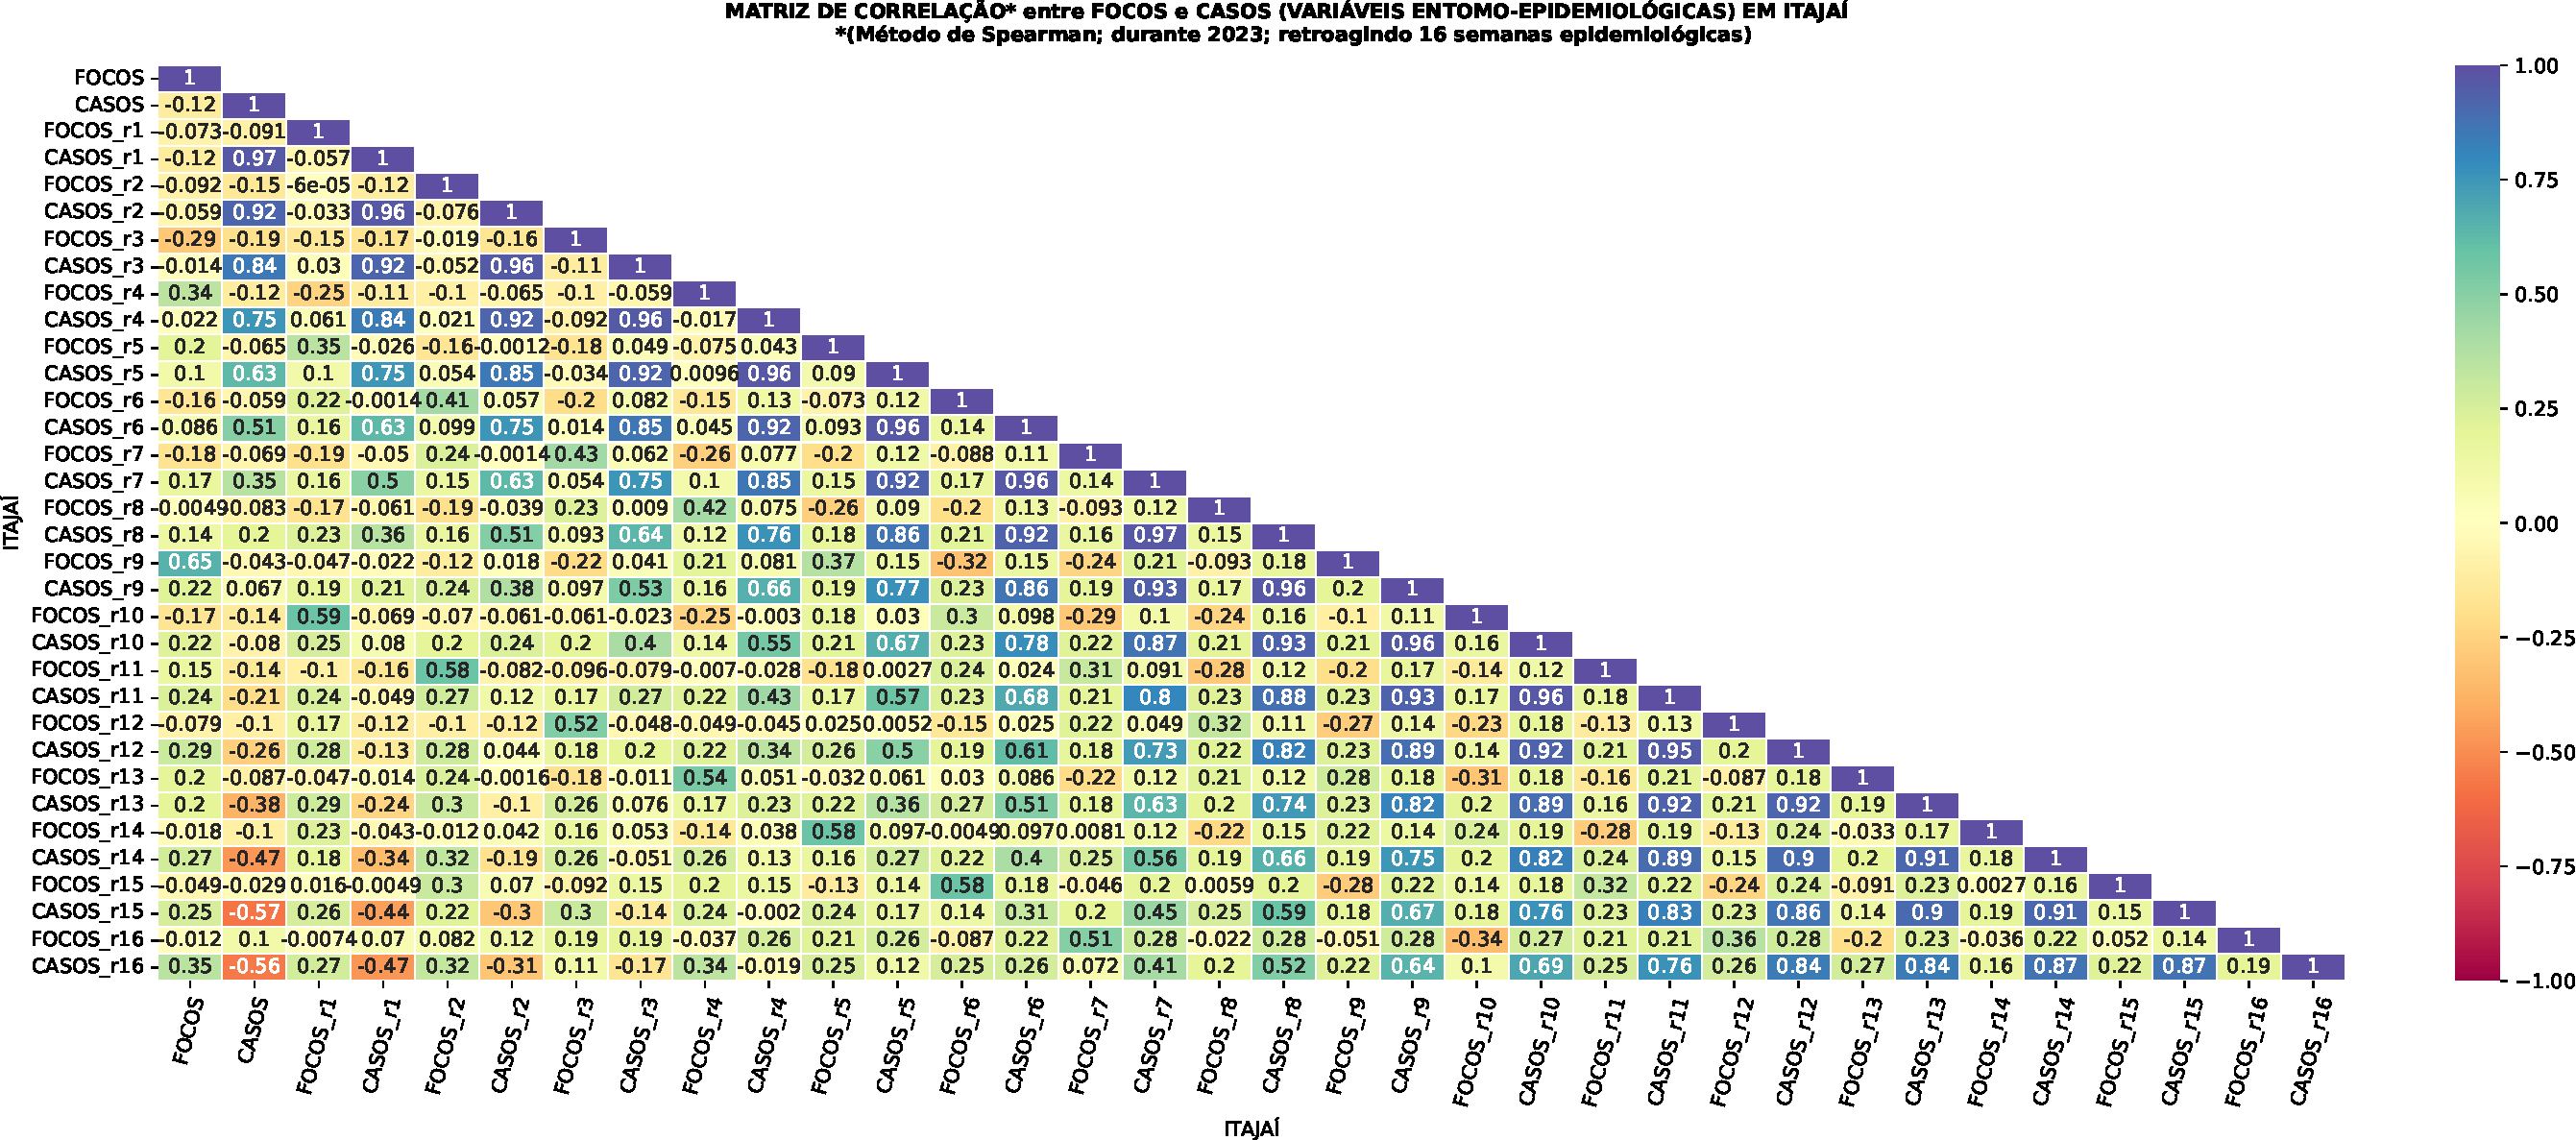
\includegraphics[width=0.47\textwidth]{figuras/matriz_correlacao_spearman_fococaso_ITAJAI_r16s_2023.pdf}
        }\hfill
    \subfloat[Joinville \label{fig: corr_DEE_JOI}]{
        \centering
        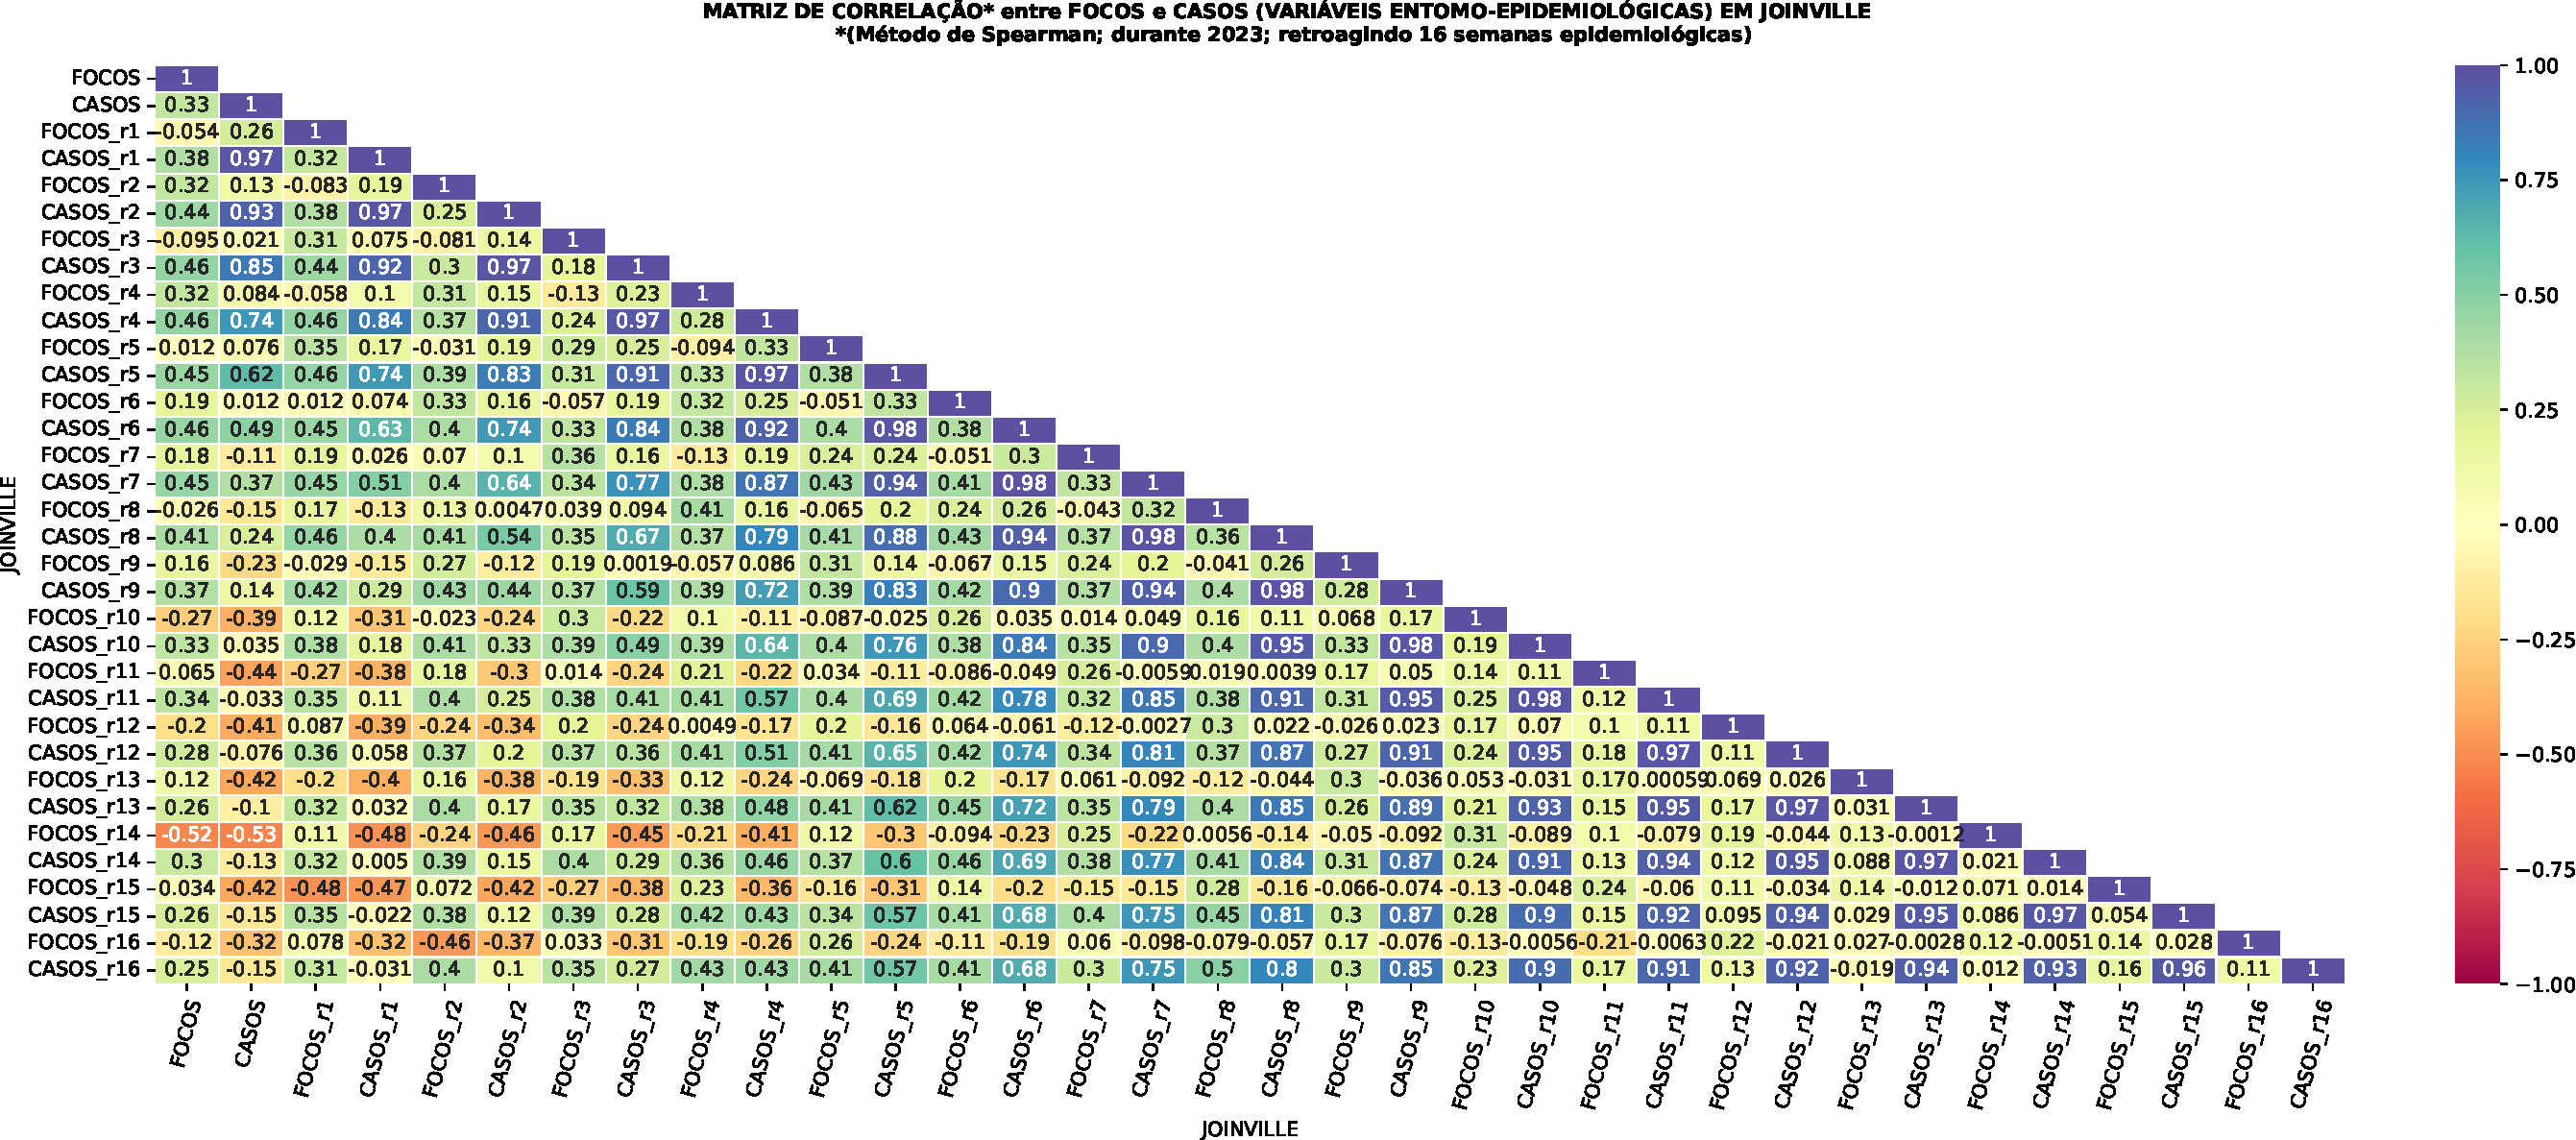
\includegraphics[width=0.47\textwidth]{figuras/matriz_correlacao_spearman_fococaso_JOINVILLE_r16s_2023.pdf}
        }
    \subfloat[Chapecó \label{fig: corr_DEE_CHA}]{
        \centering
        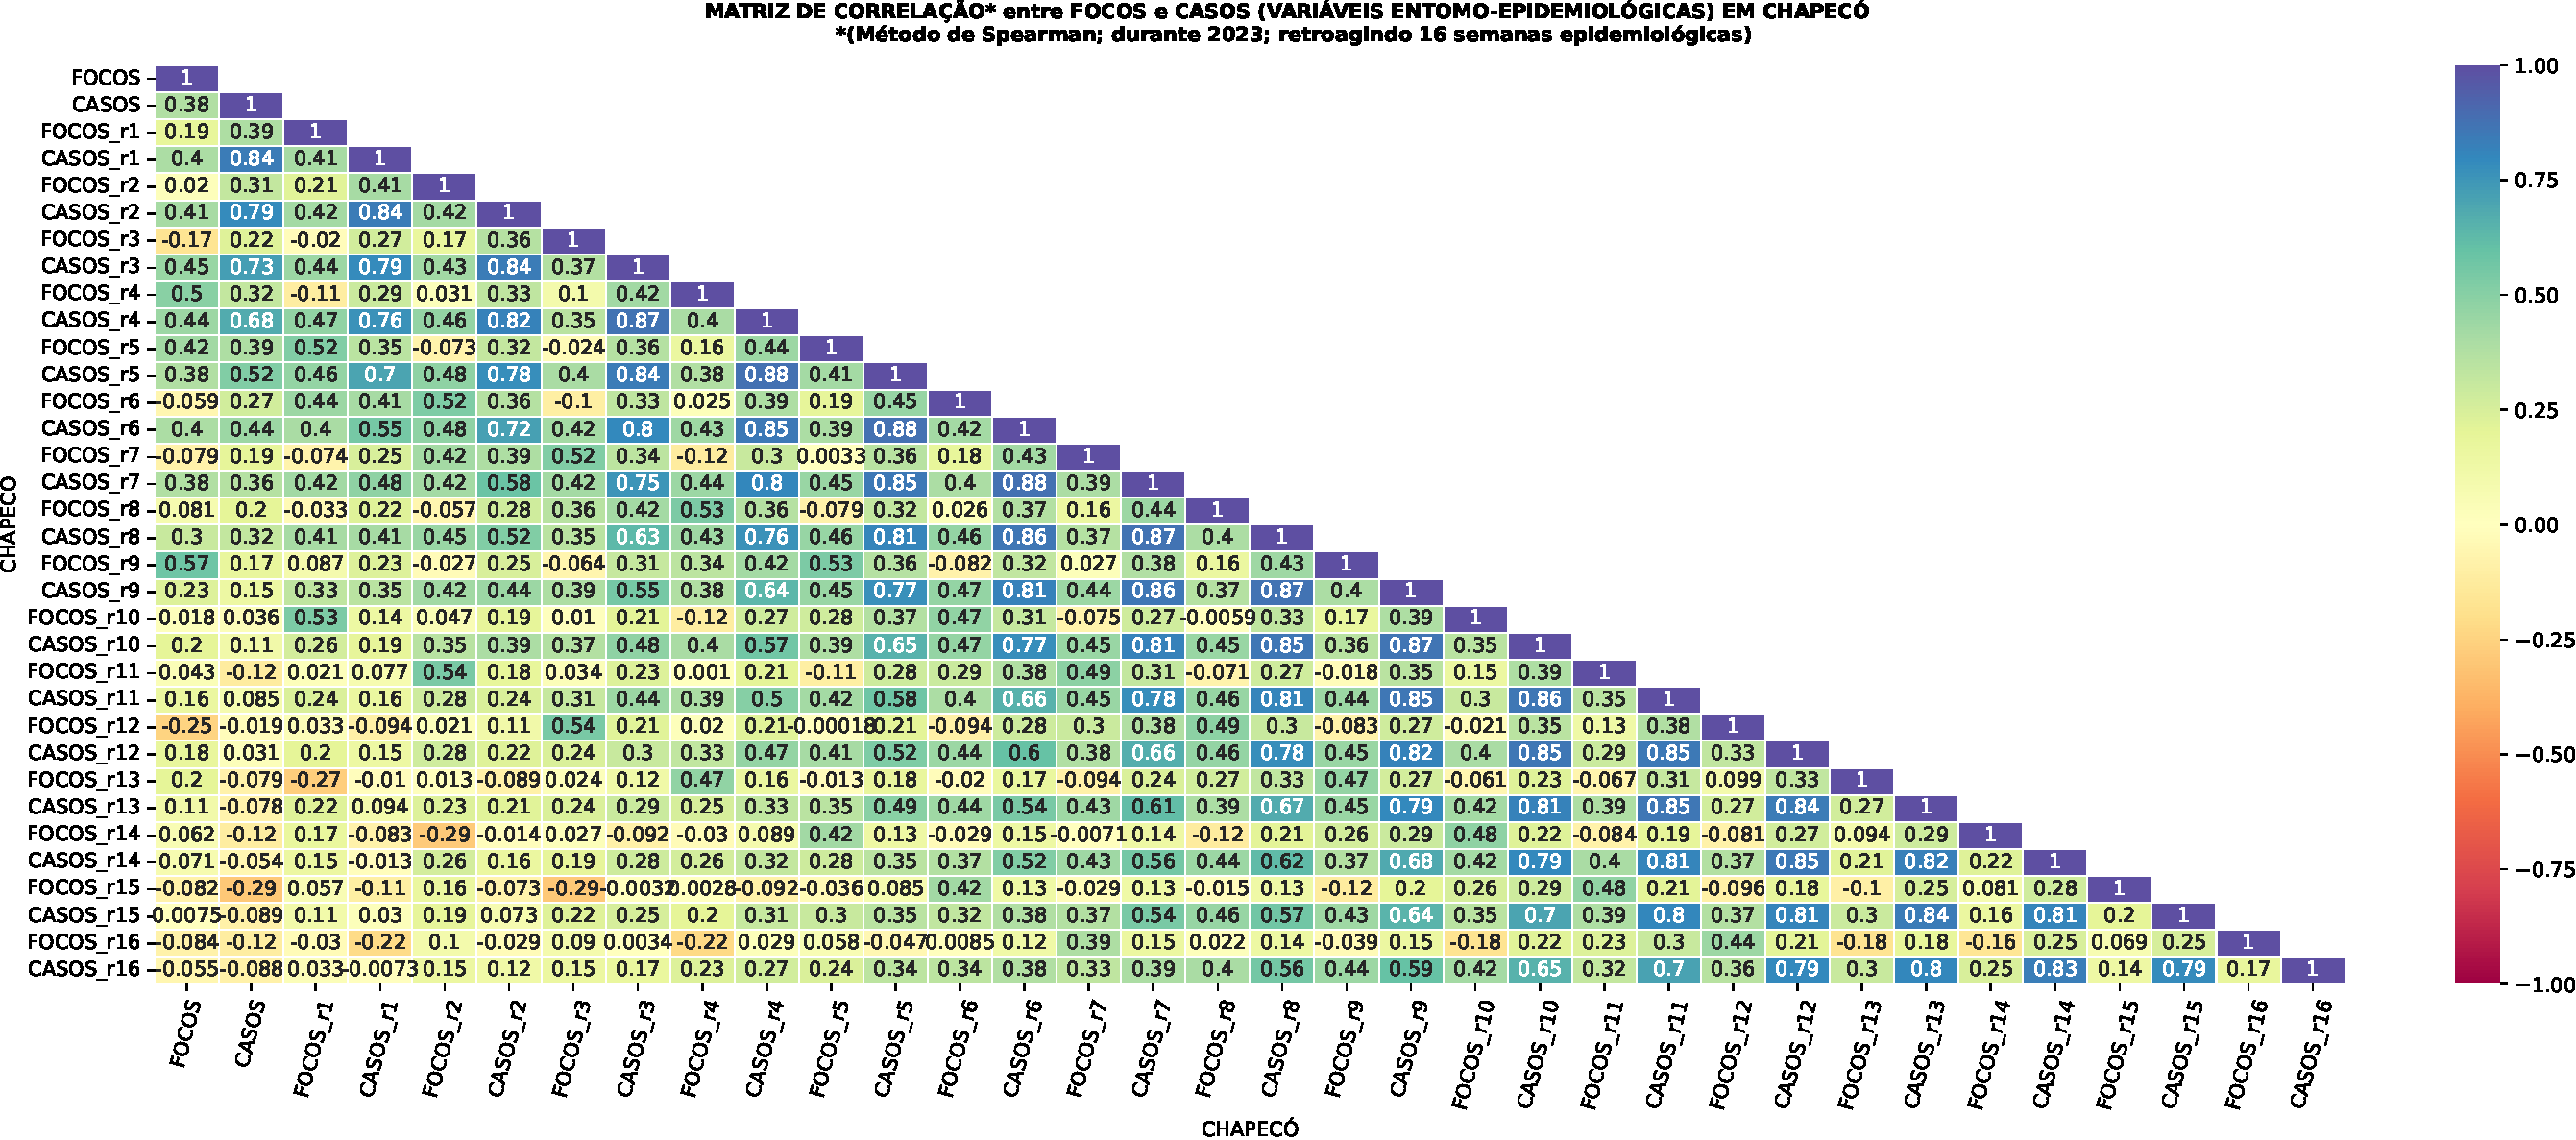
\includegraphics[width=0.47\textwidth]{figuras/matriz_correlacao_spearman_fococaso_CHAPECO_r16s_2023.pdf}
        }\hfill
    \small{Fonte: Elaboração própria (2024).}
\end{figure}

Há flutuação entre os anos, porém ao correlacionar a série temporal integralmente (figura \ref{fig: matriz_corr_DEEtotal}), os municípios de Florianópolis (figura \ref{fig: corr_DEE_FLOtotal}) e Joinville (figura \ref{fig: corr_DEE_JOItotal}) apresentaram valores médios (entre 0,5 e 0,7) e altos (entre 0,7 e 1) de correlação em quase a totalidade da análise. Os municípios de Itajaí figura \ref{fig: corr_DEE_ITAtotal}) e Chapecó figura \ref{fig: corr_DEE_CHAtotal}) apresentaram valores baixos e médios, sendo apenas altos quando correlacionados com a própria variável pretérita.  \textcolor{red}{Por quê? Pode ser indicativo que esses municípios, Florianópolis e Joinville, apresentem relação de casos de dengue autóctones maior; enquanto outros municípios, como Chapecó e Itajaí, tenham importação de casos de dengue dentro da série temporal?}

\indent Citar essa classificação da correlação na metodologia. Sugerir própria classificação: baixa, média, alta (e altíssima).

% Rumsey, D. J. (2023, 6 de fevereiro). What is r value correlation? Dummies. https://www.dummies.com/article/academics-the-arts/math/statistics/how-to-interpret-a-correlation-coefficient-r-169792/

\begin{figure}[htbp]
    \centering
    \caption{Matriz de correlações entre focos de \latim{Aedes} sp. e casos de dengue de alguns municípios catarinenses durante a série histórica, método de Spearman.}
    \label{fig: matriz_corr_DEEtotal}
    \subfloat[Florianópolis \label{fig: corr_DEE_FLOtotal}]{
        \centering
        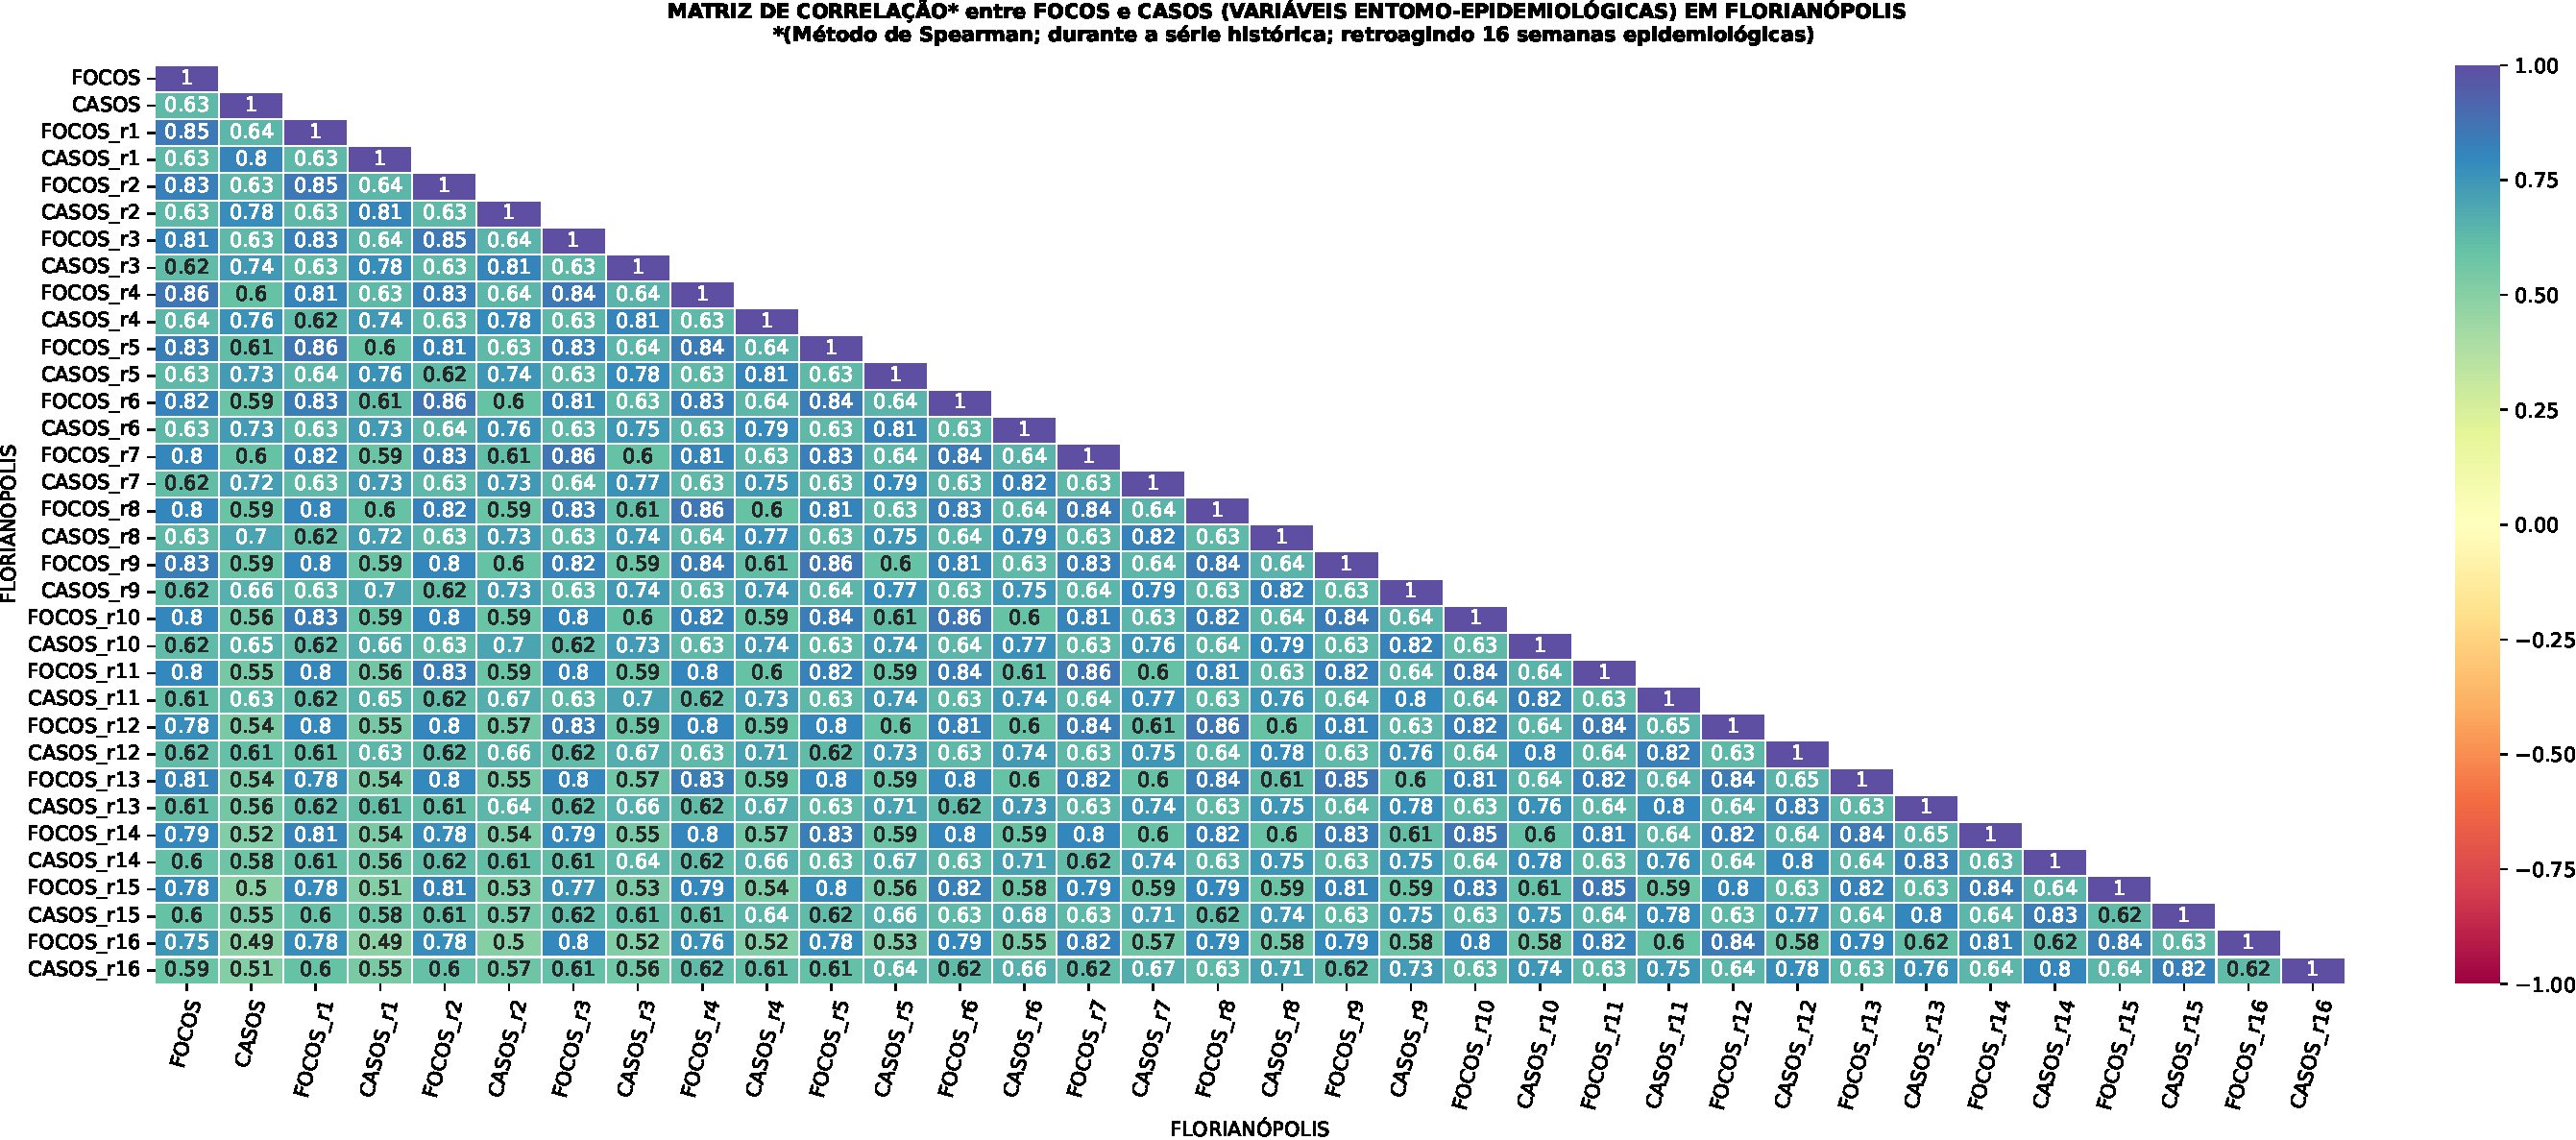
\includegraphics[width=0.47\textwidth]{figuras/matriz_correlacao_spearman_fococaso_FLORIANOPOLIS_r16s_total.pdf}
        }
    \subfloat[Itajaí \label{fig: corr_DEE_ITAtotal}]{
        \centering
        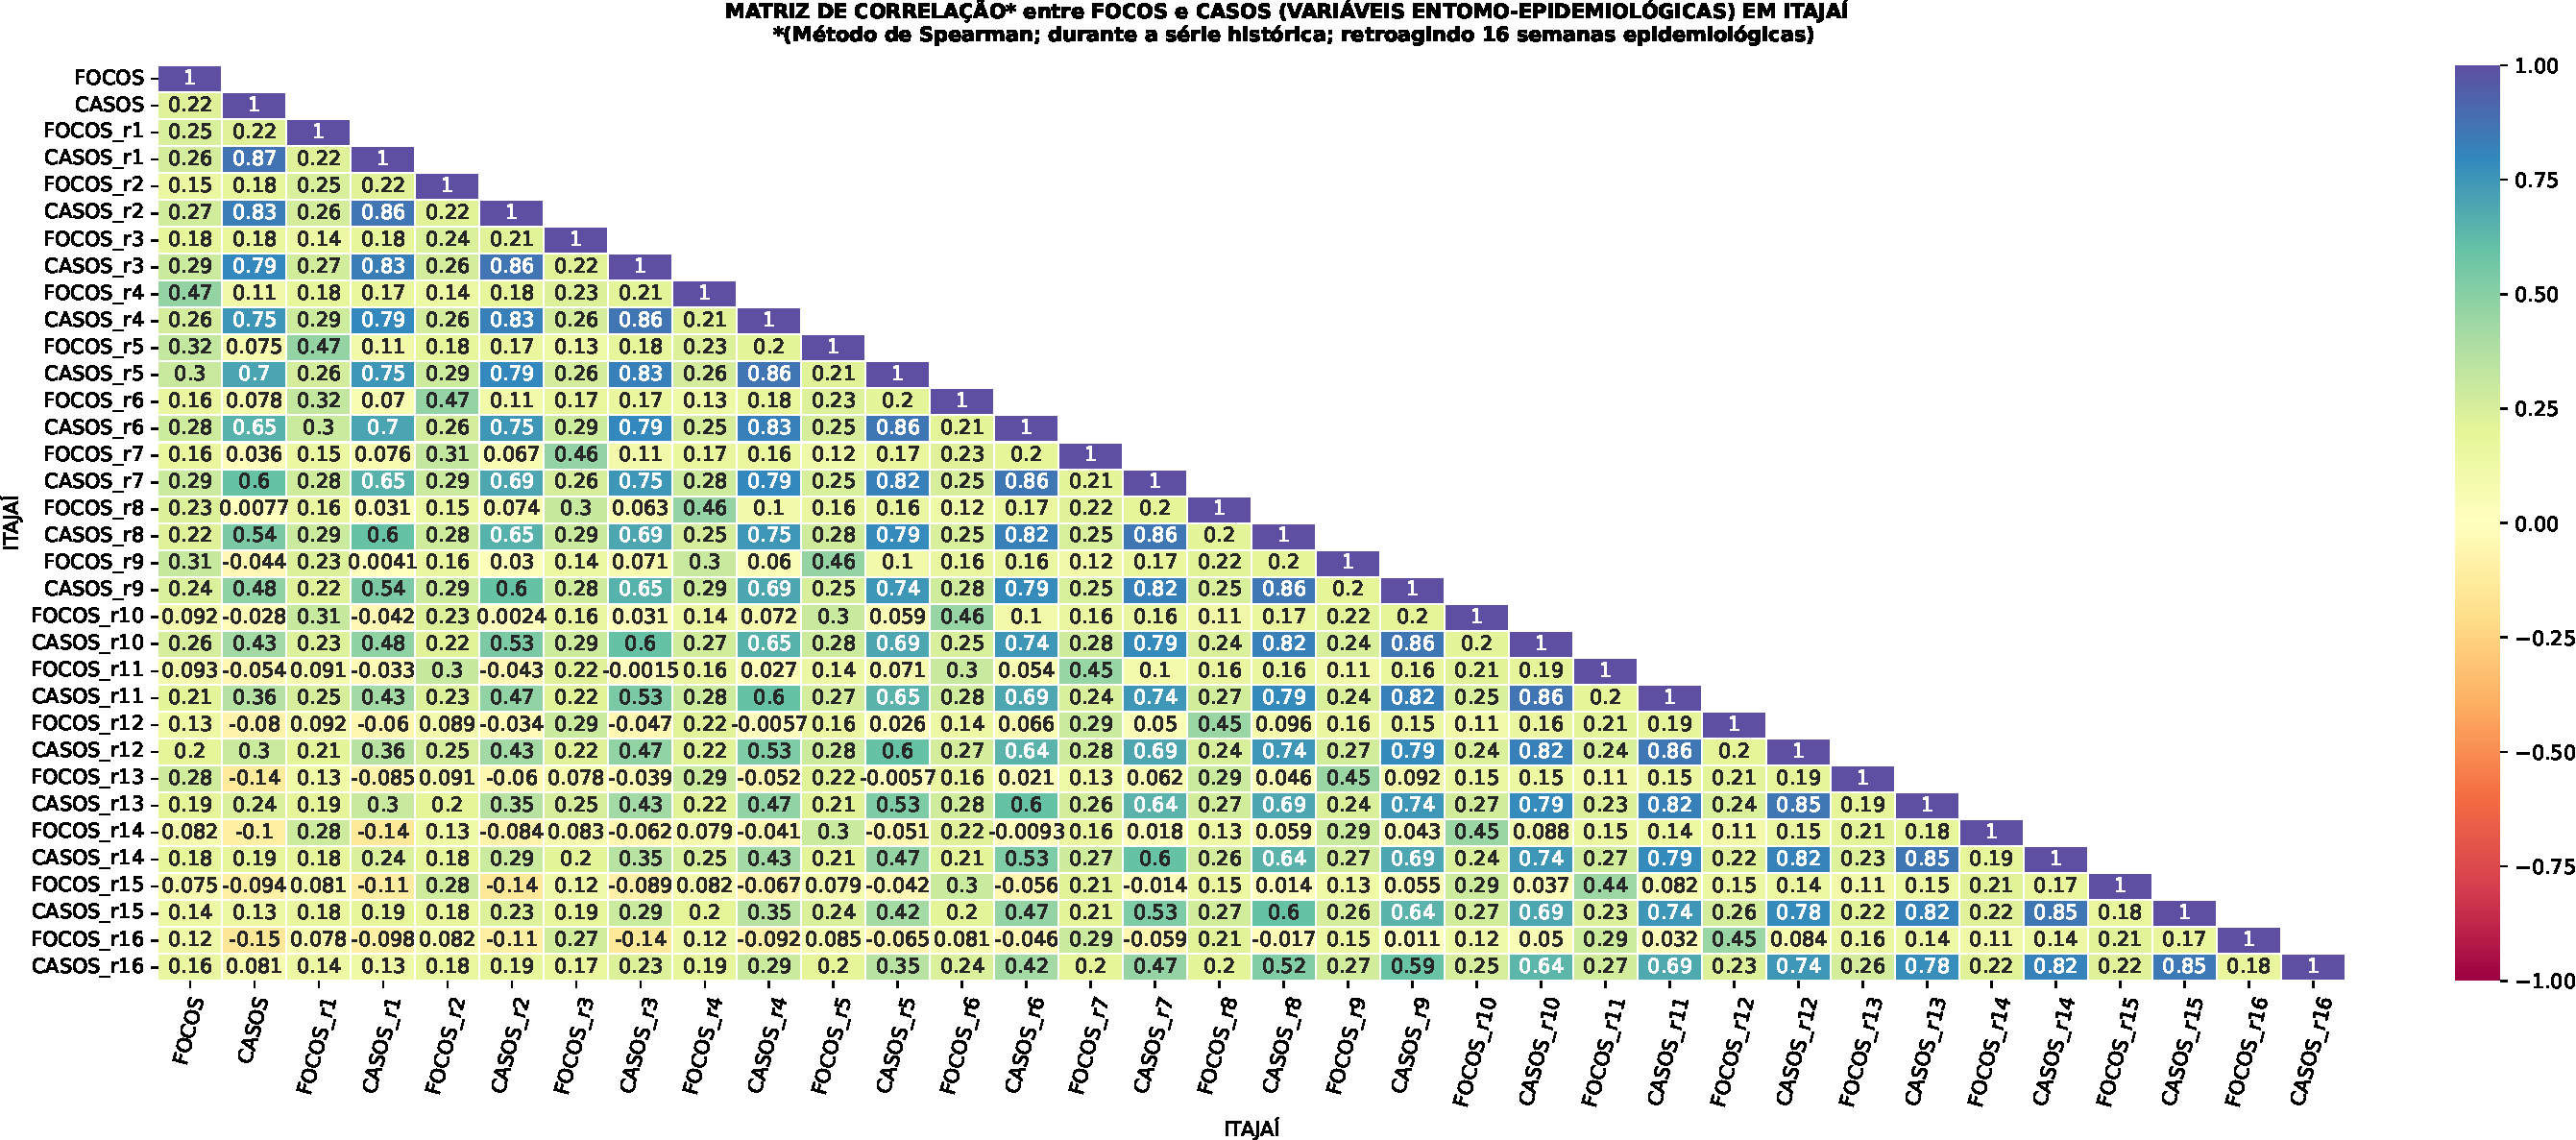
\includegraphics[width=0.47\textwidth]{figuras/matriz_correlacao_spearman_fococaso_ITAJAI_r16s_total.pdf}
        }\hfill
    \subfloat[Joinville \label{fig: corr_DEE_JOItotal}]{
        \centering
        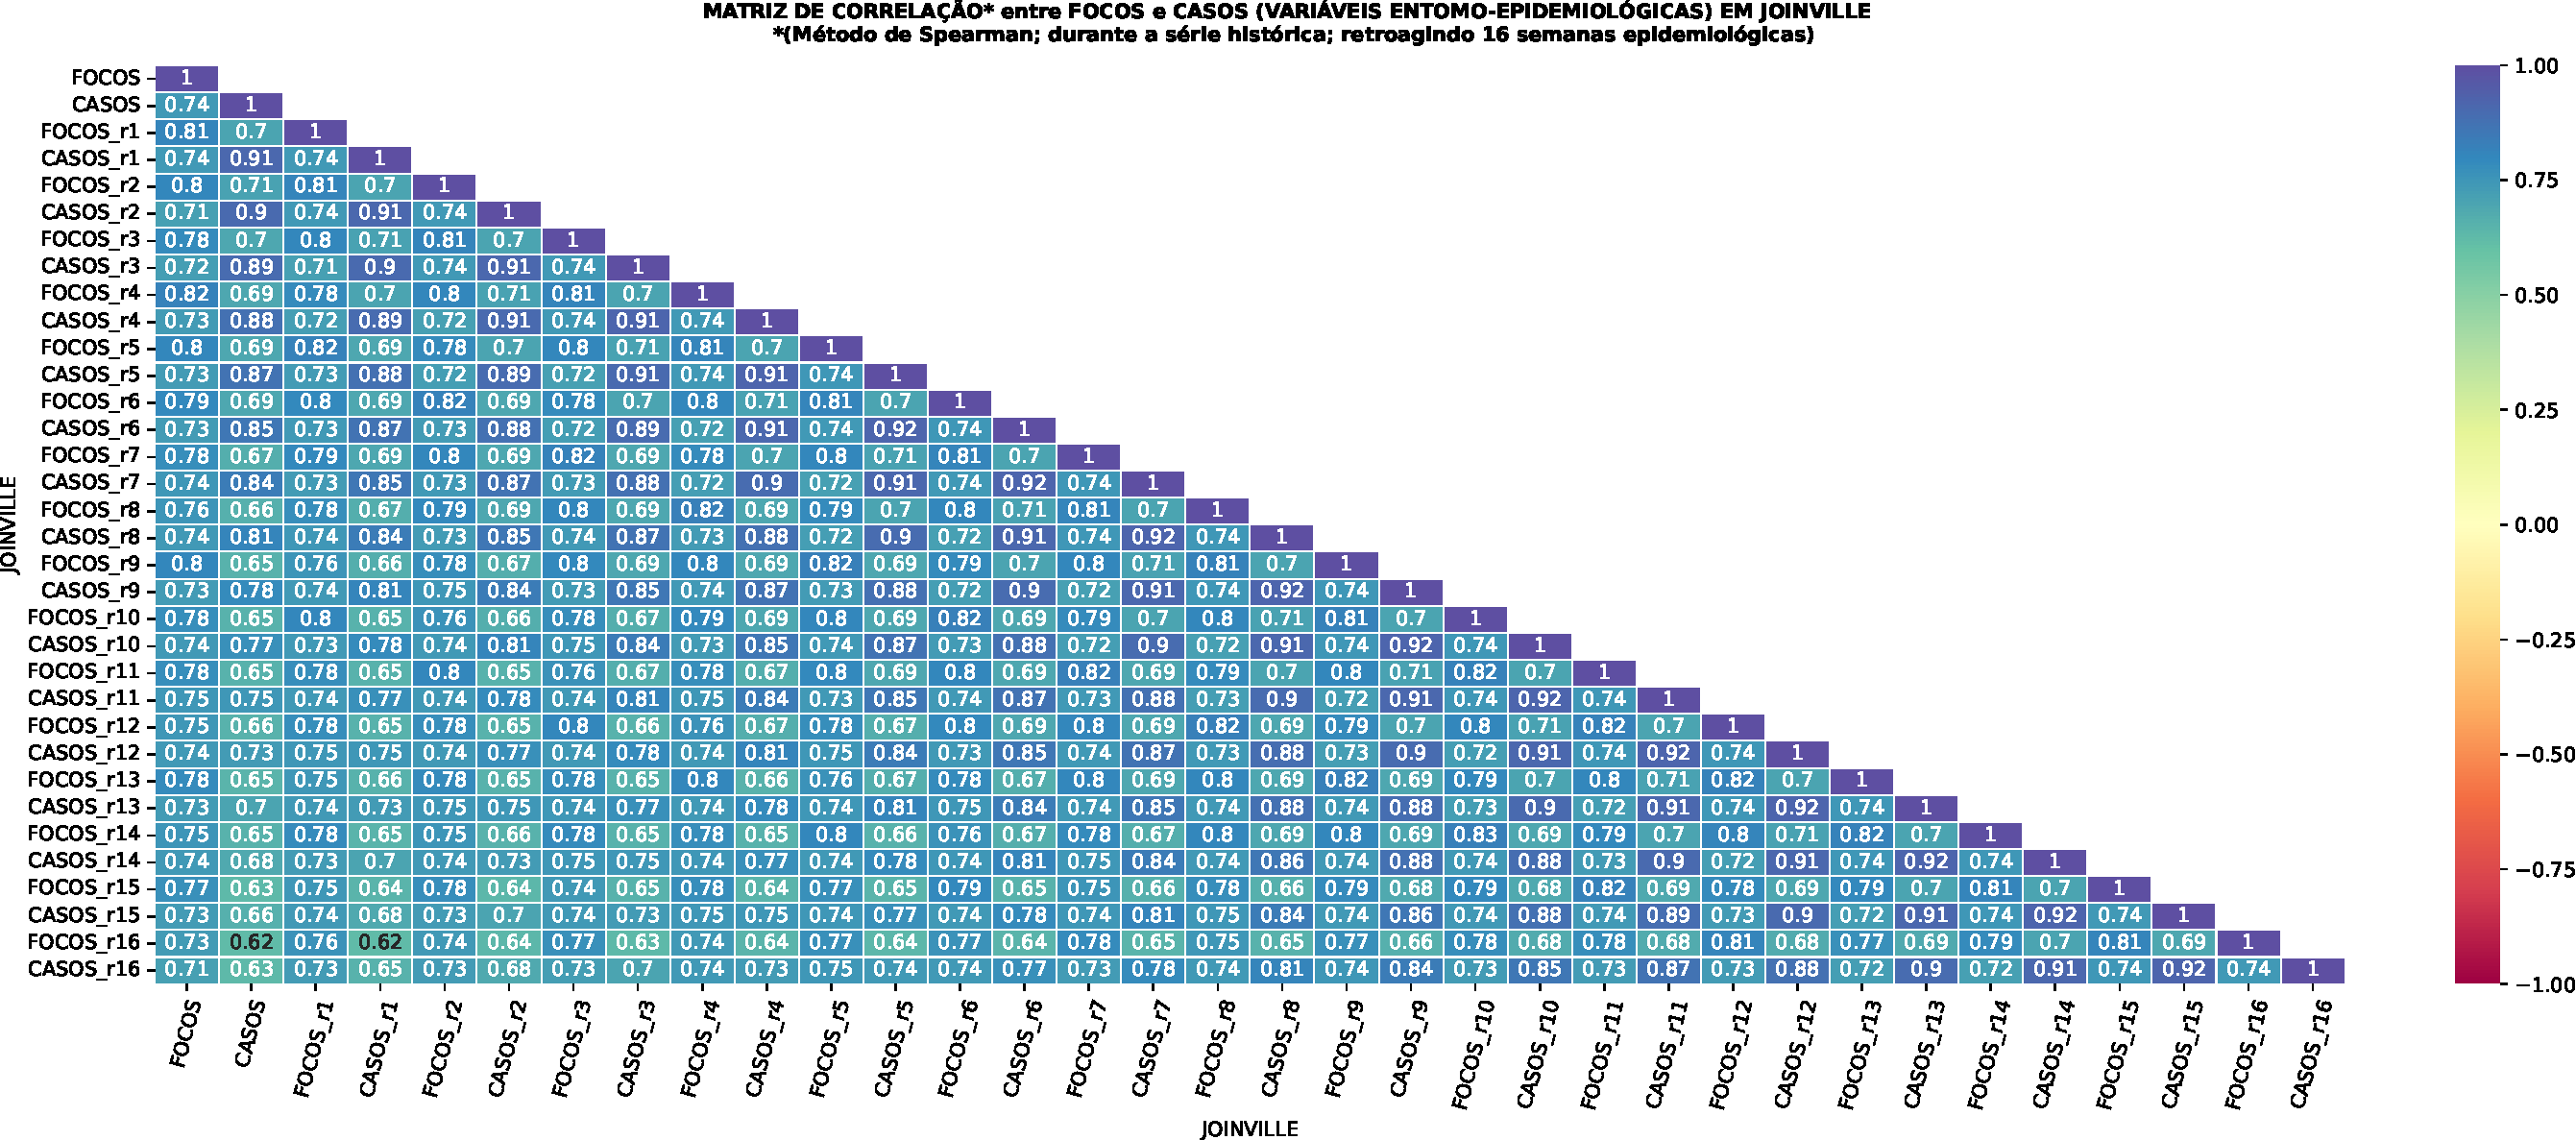
\includegraphics[width=0.47\textwidth]{figuras/matriz_correlacao_spearman_fococaso_JOINVILLE_r16s_total.pdf}
        }
    \subfloat[Chapecó \label{fig: corr_DEE_CHAtotal}]{
        \centering
        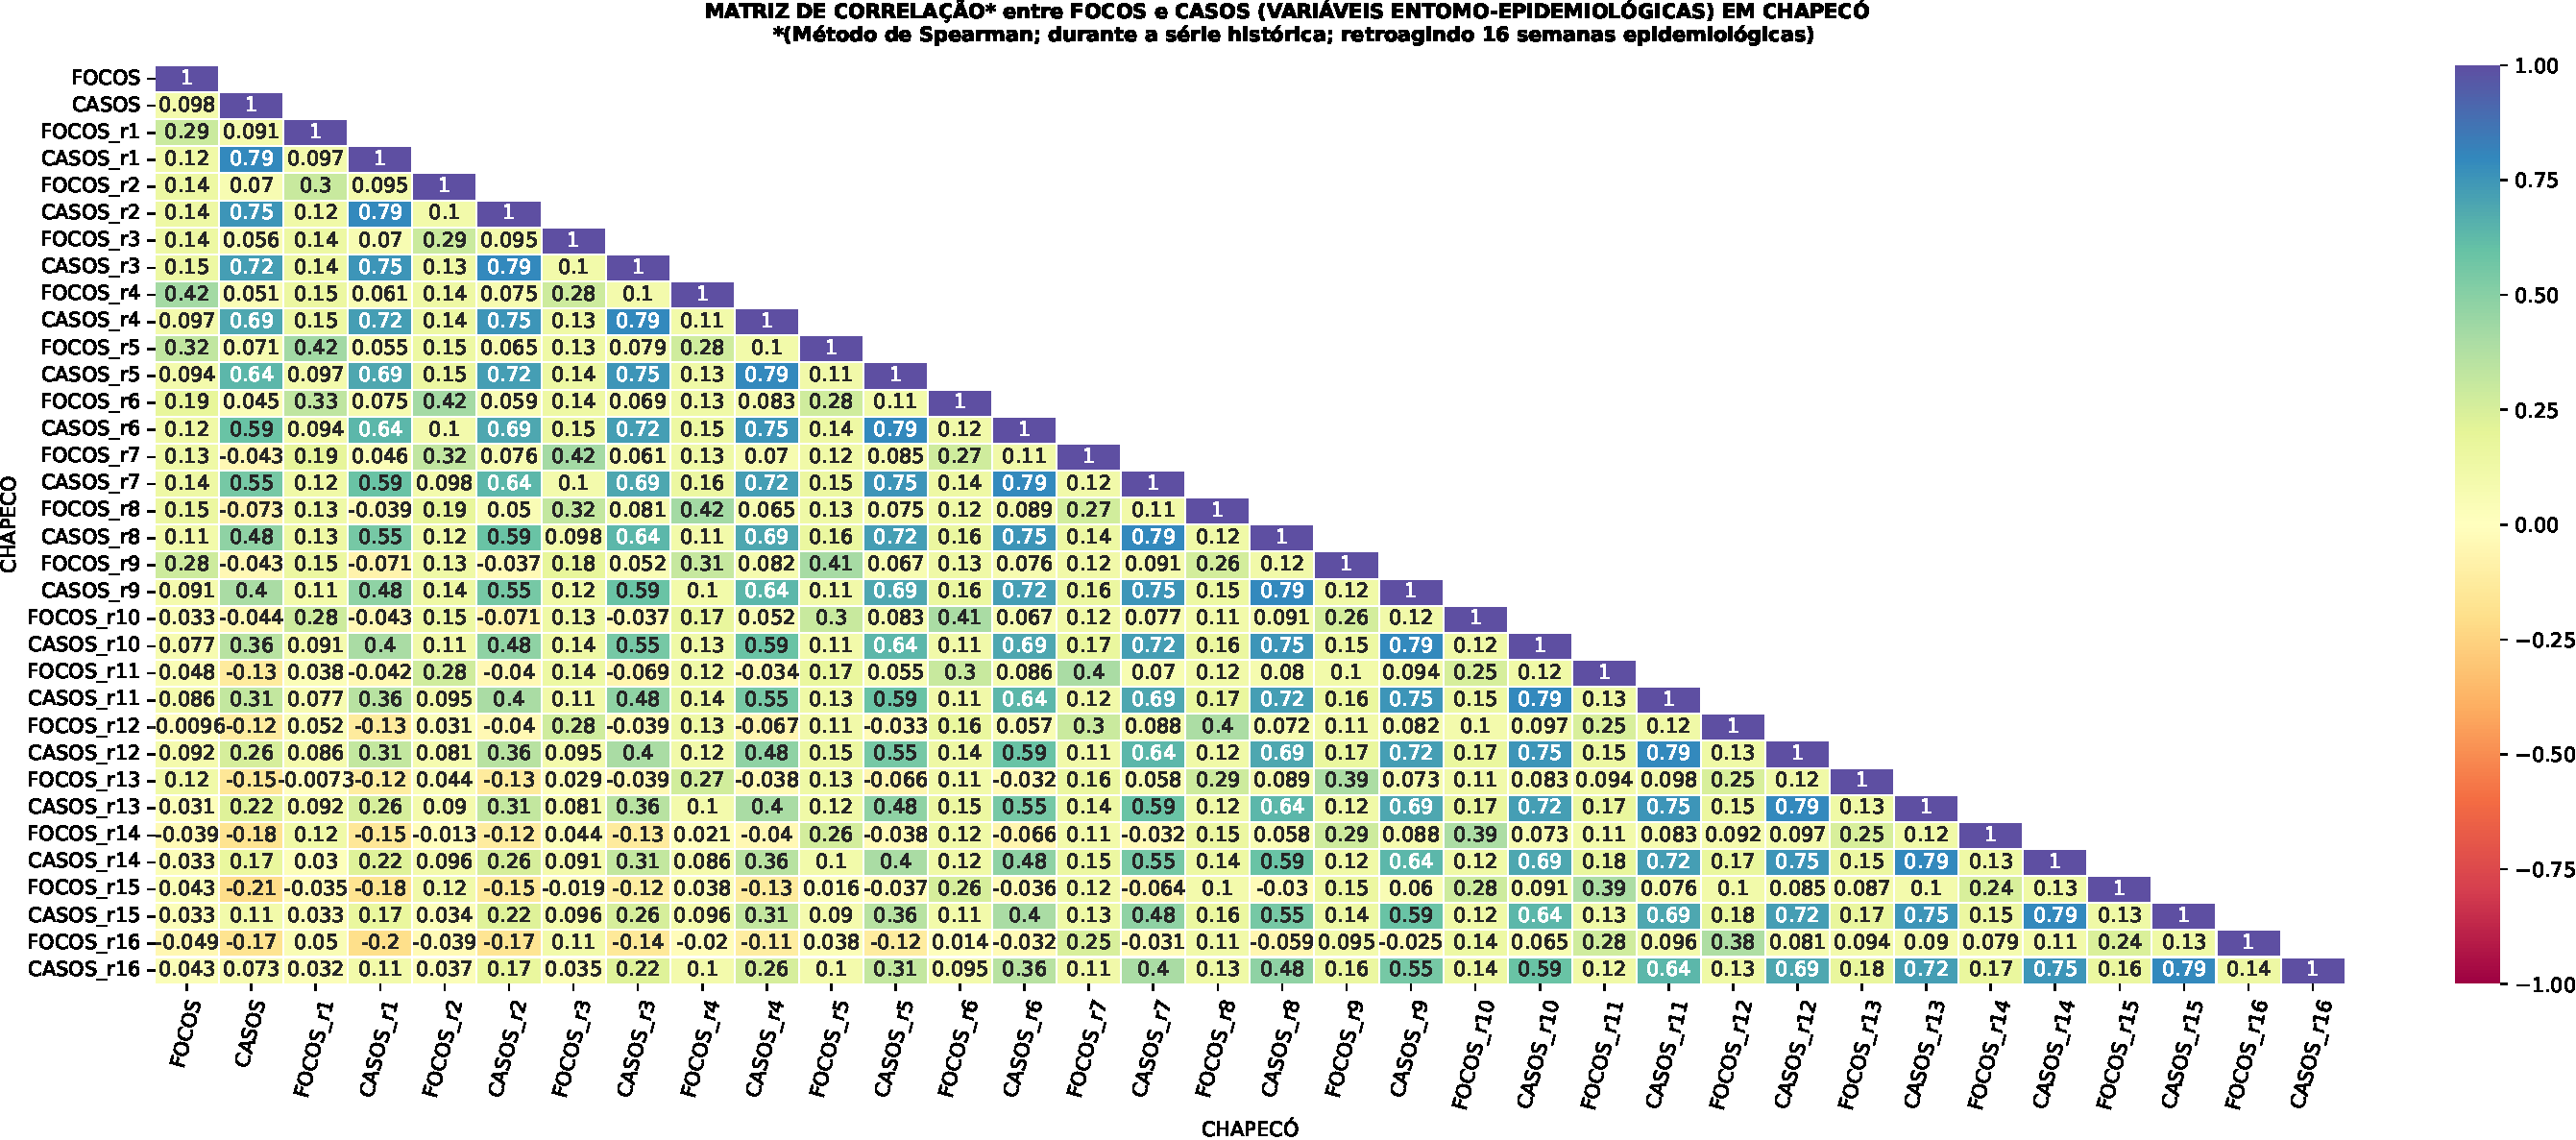
\includegraphics[width=0.47\textwidth]{figuras/matriz_correlacao_spearman_fococaso_CHAPECO_r16s_total.pdf}
        }\hfill
    \small{Fonte: Elaboração própria (2024).}
\end{figure}

% entre esses elementos citados anteriormente e os \acrshort{DEC} (precipitação e temperaturas mínima, média e máxima)
\indent A correlação entre os \acrshort{DEE} (focos de \latim{Aedes} sp. e casos de dengue) e os \acrshort{DEC} (precipitação e temperaturas mínima, média e máxima) também foram realizadas pelo método de Spearman durante cada ano citado anteriormente (de 2020 a 2023) e a série histórica. Apenas duas variáveis climatológicas, temperatura média e precipitação, foram retroagidas 16 semanas epidemiologicas. A temperatura média foi a escolhida para retroação pois, nas quatro (4) cidades, as correlaçãos entre ela e as temperaturas mínima e máxima se apresentaram altas. Também apenas apresentaremos essas análises realizadas no ano de 2023 (figura \ref{fig: matriz_corr_CLI}). Também há flutuação entre os anos, porém ao correlacionar a série temporal integralmente, apenas as variáveis climatológicas entre si apresentaram valores médios (entre 0,5 e 0,7) e altos (entre 0,7 e 1) de correlação.

\begin{figure}[htbp]
    \centering
    \caption{Matriz de correlações entre focos de \latim{Aedes} sp., casos de dengue e variáveis climatológicas de alguns municípios catarinenses durante 2023, método de Spearman.}
    \label{fig: matriz_corr_CLI}
    \subfloat[Florianópolis \label{fig: corr_CLI_FLO}]{
        \centering
        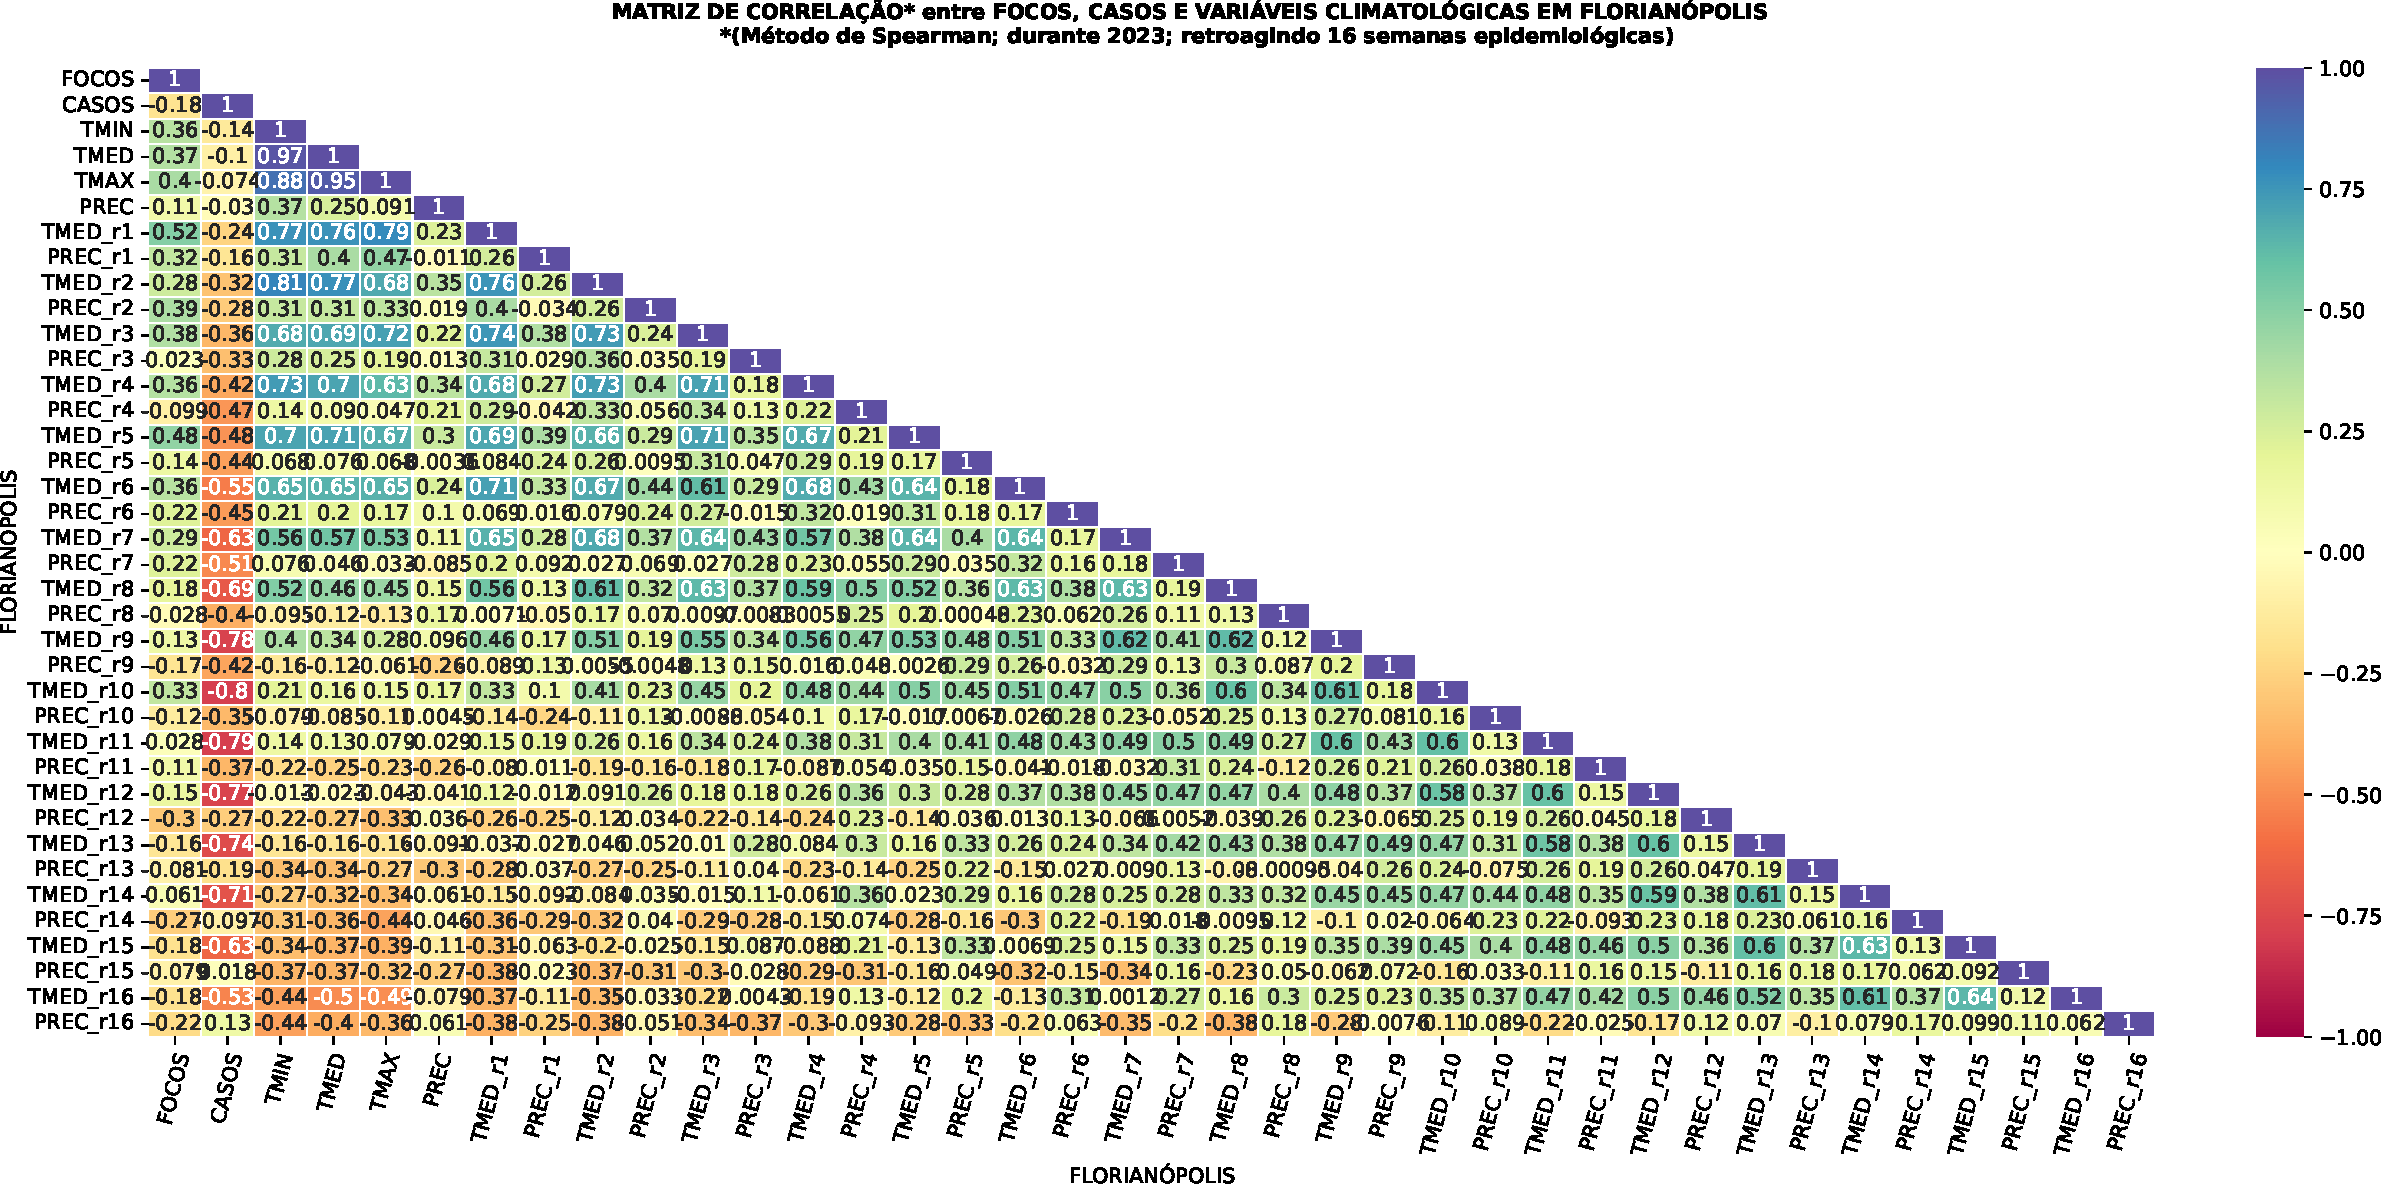
\includegraphics[width=0.47\textwidth]{figuras/matriz_correlacao_spearman_FLORIANOPOLIS_r16s_2023.pdf}
        }
    \subfloat[Itajaí \label{fig: corr_CLI_ITA}]{
        \centering
        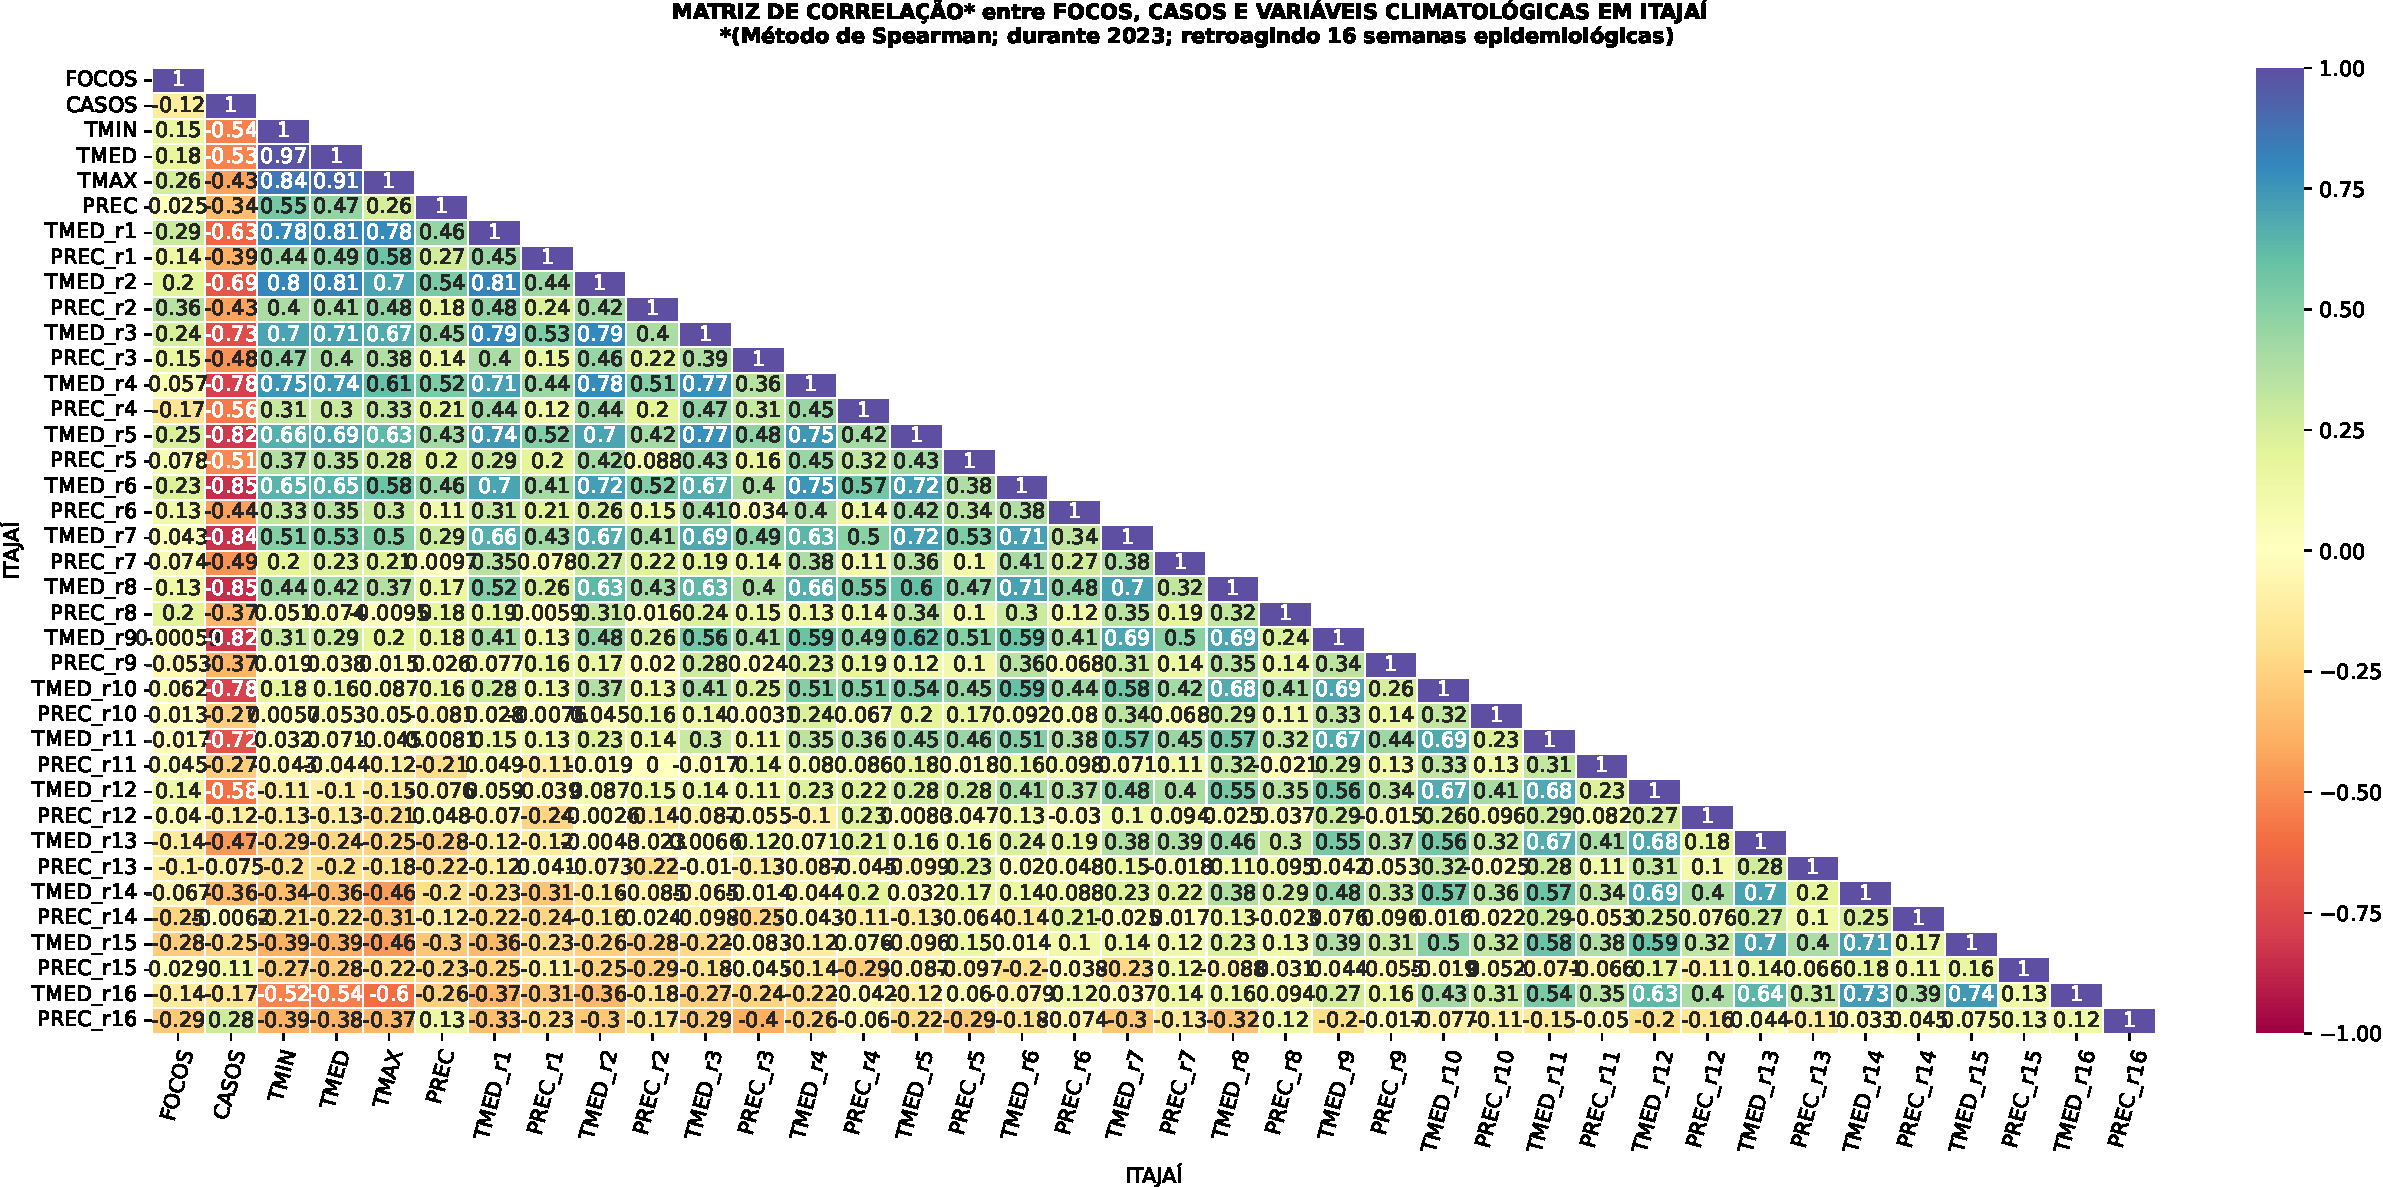
\includegraphics[width=0.47\textwidth]{figuras/matriz_correlacao_spearman_ITAJAI_r16s_2023.pdf}
        }\hfill
    \subfloat[Joinville \label{fig: corr_CLI_JOI}]{
        \centering
        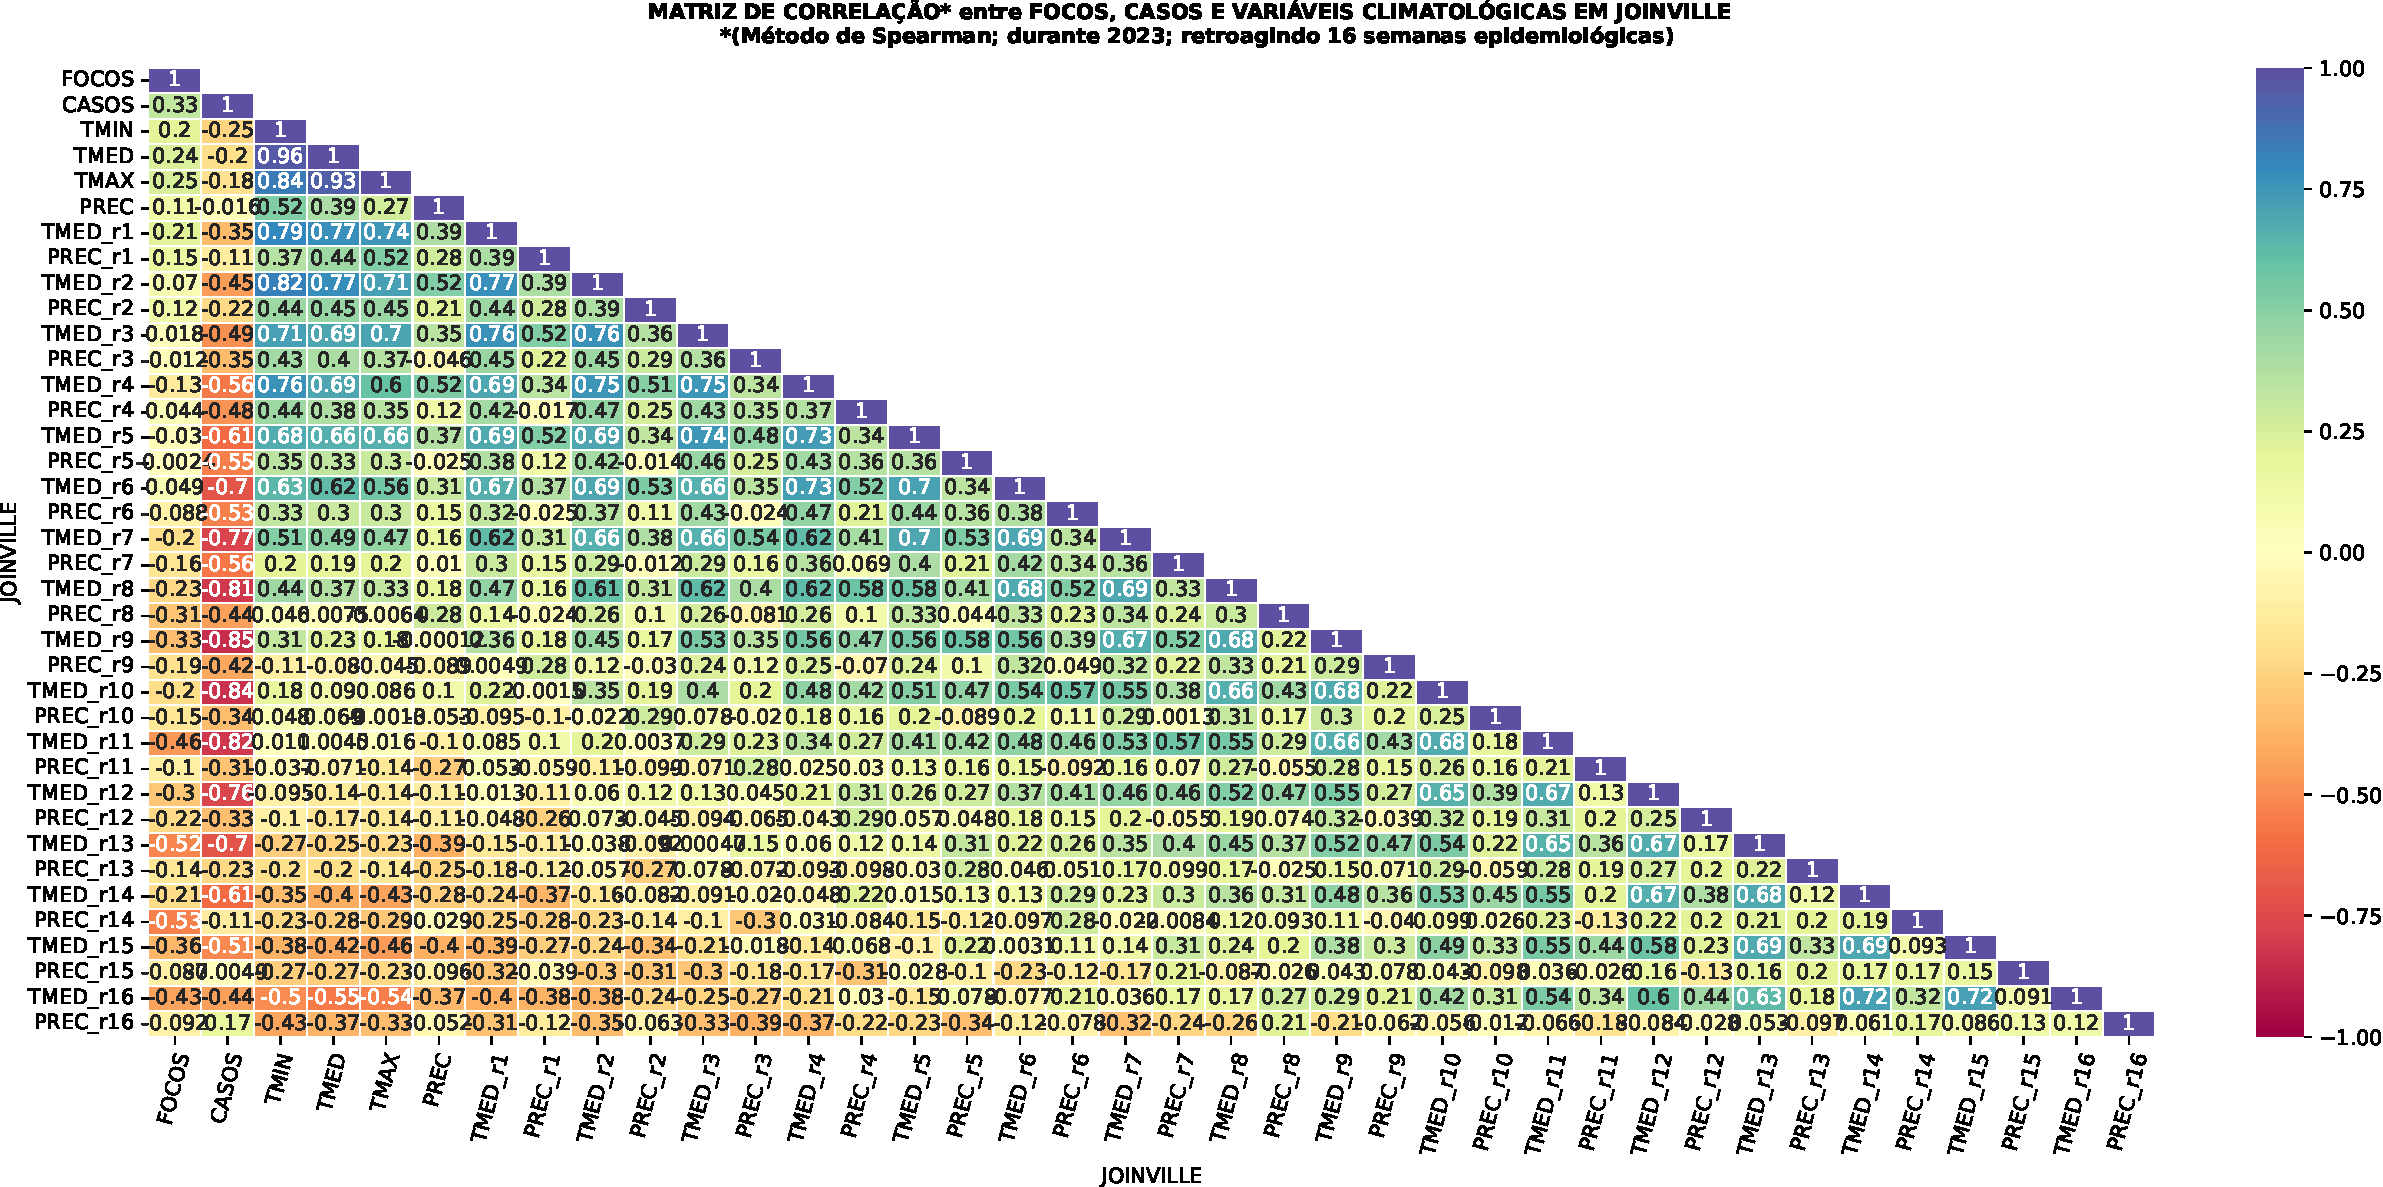
\includegraphics[width=0.47\textwidth]{figuras/matriz_correlacao_spearman_JOINVILLE_r16s_2023.pdf}
        }
    \subfloat[Chapecó \label{fig: corr_CLI_CHA}]{
        \centering
        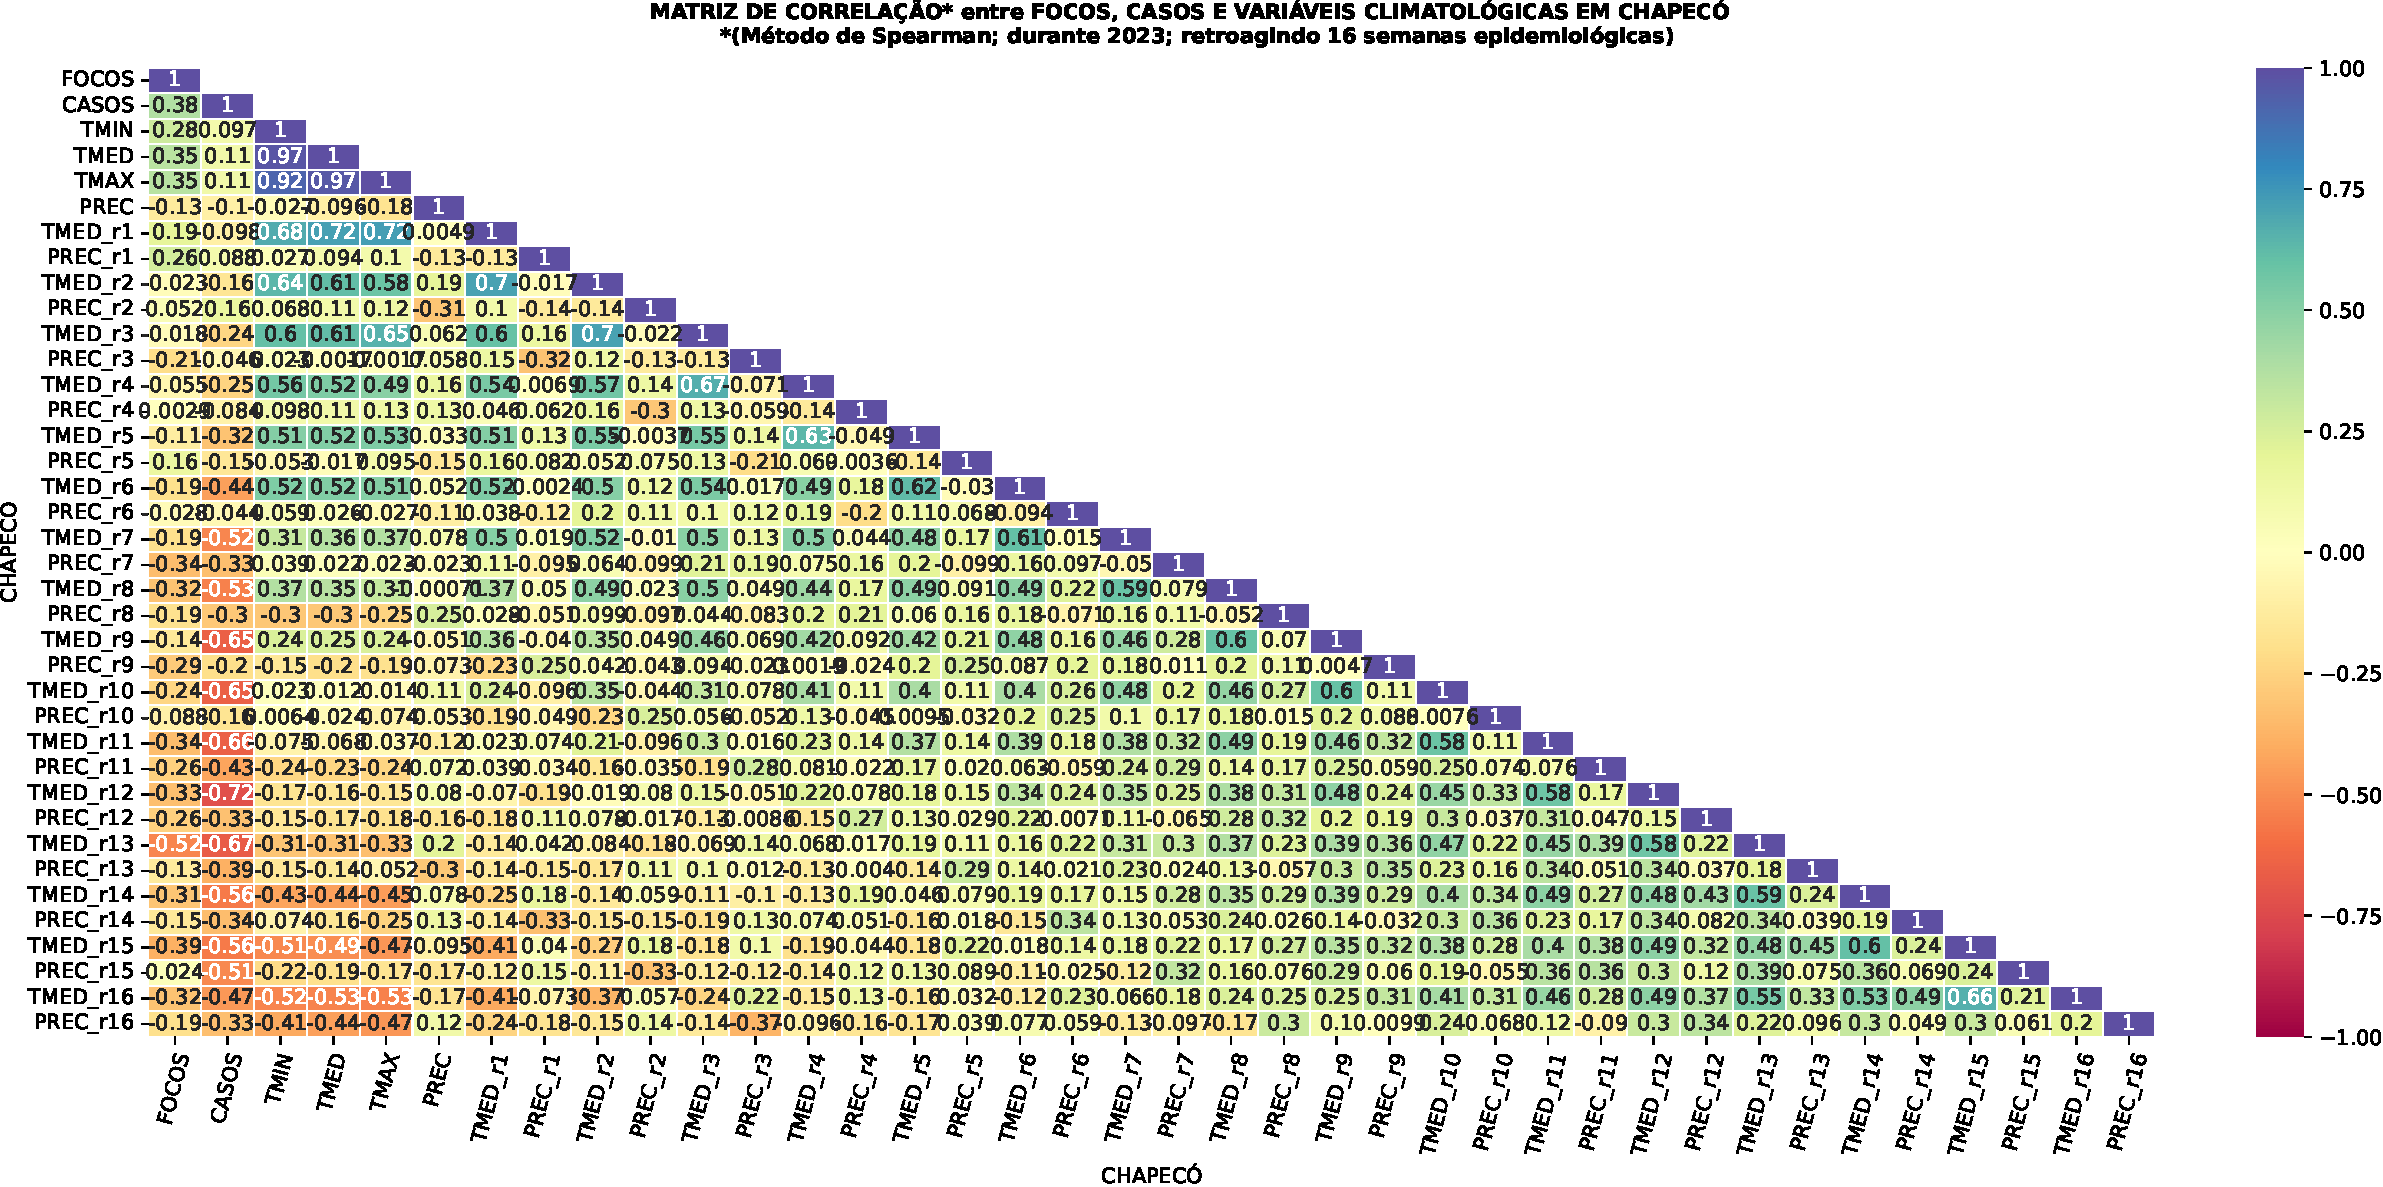
\includegraphics[width=0.47\textwidth]{figuras/matriz_correlacao_spearman_CHAPECO_r16s_2023.pdf}
        }\hfill
    \small{Fonte: Elaboração própria (2024).}
\end{figure}

% E entre os \acrshort{DEE} e limiares dos \acrshort{DEC}.
\indent 






% \begin{figure}[H]
%     \centering
%     \caption{Número de focos de \ingles{Aedes aegypti} e casos de dengue em Santa Catarina nos anos de 2020 e 2021, segundo o Boletim Epidemiológico nº 33 da \acrshort{Dive}.} %LEGENDA DA IMAGEM GLOBAL
%     \label{fig:focoscasos20-21}
%     \subfloat[Número de focos de \ingles{Aedes aegypti} em 2020 e 2021 no Estado de Santa Catarina. \label{fig:focos20-21}]{
%     \includegraphics[width=0.8\textwidth]{figuras/focos_20-21.png}
%     }\hfill
%     \subfloat[Número de casos de dengue em 2020 e 2021 no Estado de Santa Catarina. \label{fig:casos20-21}]{
%     \includegraphics[width=0.8\textwidth]{figuras/casos_20-21.png}
%     }\\
%     \small{Fonte: \cite{DiveDENGUE}.}
% \end{figure}




\indent A rede neural apresentou baixo ajuste frente ao comportamento dos fenômenos.

\indent \textcolor{red}{explicar como evitar "double dipping".}



\indent Inicialmente, foram utilizados os pacotes \ingles{pandas}, \ingles{numpy} e \ingles{sklearn} \cite{scikit-learn_2011_pedregosa, sklearn_2013_buitinck}. Dessa maneira, os conjuntos de dados entomo-epidemiológicos e climatológicos foram estruturados em um único arranjo de dados para cada município. Essa estrutura foi composta pela variável dependente (entomológica ou epidemiológica) e por variáveis explicativas (elementos climáticos). Esse arranjo só foi possível com municípios que apresentavam todos os conjuntos de dados presentes. Sendo a variável dependente epidemiológica, é incluída a variável entomológica como explicativa. A configuração final do arranjo assumia, entre a variável dependente e as explicativas, horizonte preditivo de quatro (4) semanas epidemiológicas e retroação de oito (8) semanas epidemiológicas. Sendo a variável dependente epidemiológica, o horizonte preditivo de duas (2) semanas epidemiológicas e retroação de três (3) semanas epidemiológicas. Dessa última configuração, as variáveis explicativas (x) e dependente (y) foram divididas em dois conjuntos: treino e teste. Também foi previamente fixado um valor de gerador de números aleatórios (\ingles{seed}).

\indent Após isso, com a utilização dos pacotes \ingles{tensorflow} \cite{tensorflow_2015_whitepaper} e \ingles{keras} \cite{keras_2015_chollet}, do próprio \ingles{tensorflow}, fez-se a instanciação do modelo de rede neural. A primeira camada incluída (camada zero (0)) faz o achatamento dos dados de entrada (variáveis explicativas). Logo, foram adicionadas duas camadas densas (camadas: um (1) e dois (2)) com dez (10) nós (neurônios) cada e ativadas por uma função \ingles{\acrshort{ReLU}} (unidade linear retificada). Então, acionou-se uma camada de regularização (camada três (3)) e uma camada densa de saída (camada 4 (4)). Essa última camada foi criada com a quantidade de nós suficientes para receber o valor de saída (variável dependente) e ativada por uma função \ingles{softmax}. Finalmente, o modelo foi compilado com otimização da taxa de aprendizagem (0,01), configuração de perda (entropia cruzada categórica esparsa) e de métrica (acurácia). Foi ajustado com 100 ciclos (épocas) máximos de treinamento e alocados 20 porcento (0,2) para validação, sendo que o número de ciclos durante a fase de treino foi limitado por um monitor de valor de perda, assim o treinamento encerra antes de 100 ciclos.

\indent Para o modelo \ingles{random forest}, utilizou-se o pacote \ingles{sklearn} e o mesmo conjunto de treino e teste das variáveis explicativas (x) e dependente (y). Ao compilar, foi atribuído um número total de árvores presentes (100) e o gerador de números aleatórios (previamente citado) para, então, ajustar aos conjuntos de treino das variáveis explicativas (x) e dependente (y).

\subsection{Pós-processamento}

\indent Os dados de casos de dengue, quando comparados entre as fontes (\acrshort{Dive} e \acrshort{DataSUS}), há diferença de atualização. Sendo os dados da própria \acrshort{Dive} mais atualizados, sendo eleitos para treinamento do modelo.

\indent Obteve-se os \ingles{shapefiles} do \acrshort{IBGE} (2022) para os limites territoriais (federal, estadual e municipais) do Estado de \acrlong{SC}. Para esse estudo, foi utilizado o recorte espacial durante a execução do prório \ingles{script}, sendo: longitude entre 54º5' e 57º5', ambas sul; e latitude entre 29º5' e 25º5', ambas oeste. Com esse recorte, pode-se evidenciar a totalidade do Estado de \acrlong{SC} e um pouco além de seus limites.

\indent Os modelos, previamente sintetizados, foram abertos através da biblioteca \ingles{joblib}, dos próprios desenvolvedores da biblioteca \ingles{sklearn}. Os dados de entrada são as próprias variáveis explicativas (x). Esses são abertos e estruturados pela biblioteca \ingles{pandas} e logo computados pela modelagem, retornando os valores de previsão da variável dependente (y).

\indent O centróide de cada município, que tenha algum valor de previsão, é incluído nesse novo conjunto de dados de retorno (previsão). O próprio centróide é padronizado ao Sistema de Referência de Coordenadas (\acrfull{CRS}) utilizado pelos \ingles{shapefiles} do \acrshort{IBGE} e o conjunto  de dados é transformado em \ingles{geodataframe} pela biblioteca \ingles{geopandas}. As semanas epidemiológicas também são transformadas em variável do tipo \ingles{datetime64[ns](YYYY-mm-dd)}.

\indent Para cada semana epidemiológica prevista, e através das bibliotecas \ingles{geopandas}, \ingles{matplotlib} e \ingles{shapely}, os valores calculados da variável dependente (y) foram atribuídos ao posicionamento geográfico de cada centróide, conforme \acrshort{CRS}, e sintetizado mapas temáticos. Um deles, o mapa temático coroplético, tem visualização e barra de legenda conforme o número previsto dos próprios municípios com modelagem. O outro, mapa temática com densidade de kernel, foi obtido através da biblioteca \ingles{seaborn}, onde é visualizado áreas de concentração da previsão, ponderando o número previsto.

\section{Validação dos Modelos}

\indent Para ambos os modelos, rede neural e \ingles{random forest}, fez-se, inicialmente, visualização gráfica dos valores observados e preditos. Essa exibição gráfica foi obtida através das bibliotecas \ingles{matplotlib} e \ingles{seaborn}.

\indent Para o modelo de rede neural, como citado anteriormente, foi estabelecido no próprio código um limitador de ciclagens, que avalia perda e acurácia dos conjuntos de treino e teste. Após o ajuste do modelo, graficamente é visualizado valores de acurácia e custo/custo do treinamento e do teste/validação e exibido em tela o resumo das camadas do modelo. Todas essas exibições foram obtidas através da própria biblioteca \ingles{keras}(\ingles{tensorflow}), \ingles{matplotlib} e \ingles{pandas}.

\indent Para o modelo \ingles{random forest}, algumas métricas foram exibidas graficamente, como: o histograma do erro com seu intervalo de confiança, cálculo do \acrfull{EMA}, da \acrfull{RQEQM}, do Viés e do \acrfull{r2}. Também foram visualizadas as variáveis com maior importância para a modelagem e, por permutação, para a predição, assim como a própria árvore de decisão. Todas as métricas foram obtidas pela biblioteca \ingles{sklearn}.

\section{Estudo de Caso}

\indent \textcolor{red}{Analisar o fenômeno durante algum ano. 2023! Utilizar como artigo!}

\indent \textcolor{red}{Ponto de inflexão (pandemia), além da relação climatológica!}

\section{Produto Técnico Tecnológico (PTT)}

\indent Como preditivo das dinâmicas entomológica de focos de \latim{Aedes} sp. e epidemiológica de casos de dengue no Estado de \acrlong{SC}, o \acrshort{PTT} resultante será:

\begin{itemize}
  \item o sistema computacional;
  \item visualização cartográfica desses resultados.
\end{itemize}

\indent O limiar temporal estipulado para previsão de focos de \latim{Aedes} sp. será de 56 dias (8 semanas epidemiológicas). Os primeiros 28 dias (4 semanas epidemiológicas) serão determinados a partir do sistema \acrshort{SAMeT}-\acrshort{MERGE}. Os demais dias/semanas epidemilógicas serão determinados através do \textcolor{red}{modelo de previsão \acrshort{GFS}.}

\indent O limiar temporal estipulado para previsão de casos de dengue será de 28 dias (4 semanas epidemiológicas). Os primeiros 14 dias (2 semanas epidemiológicas) serão determinados a partir do sistema \acrshort{SAMeT}-\acrshort{MERGE}. Os demais dias/semanas epidemiológicas serão determinados através do \textcolor{red}{modelo de previsão \acrshort{GFS}.}


%https://cdn.embedly.com/widgets/media.html?src=https%3A%2F%2Fwww.youtube.com%2Fembed%2F3tiuRHuzST4&display_name=YouTube&url=https%3A%2F%2Fwww.youtube.com%2Fwatch%3Fv%3D3tiuRHuzST4&image=http%3A%2F%2Fi.ytimg.com%2Fvi%2F3tiuRHuzST4%2Fhqdefault.jpg&key=40cb30655a7f4a46adaaf18efb05db21&type=text%2Fhtml&schema=youtube



\begin{longtable}[htbp]{llcrr}
\label{tab:primeiros_focos}

\caption{Primeiros registros de focos de \textit{Aedes} sp. em municípios catarinenses.} \\
\hline
\rowcolor{darkgray} \textcolor{white}{Semana} & \textcolor{white}{Município} & \textcolor{white}{Focos} & \textcolor{white}{Latitude} & \textcolor{white}{Longitude} \\
\hline
\endfirsthead

\caption{(Continuação) Primeiros registros de focos de \textit{Aedes} sp. em municípios catarinenses.} \\
\rowcolor{darkgray} \textcolor{white}{Semana} & \textcolor{white}{Município} & \textcolor{white}{Focos} & \textcolor{white}{Latitude} & \textcolor{white}{Longitude} \\
\hline
\endhead

\hline
\textit{Continua na próxima página}
\hline 
\endfoot

\hline
\textit{Finalização da tabela} \\
\hline
\endlastfoot

2012-01-01 & BALNEÁRIO CAMBORIÚ & 2 & -27.004737 & -48.621741 \\
2012-01-01 & BLUMENAU & 1 & -26.885767 & -49.097309 \\
2012-01-01 & BOMBINHAS & 2 & -27.173256 & -48.517487 \\
2012-01-01 & CHAPECÓ & 1 & -27.125144 & -52.650339 \\
2012-01-01 & FLORIANÓPOLIS & 1 & -27.577834 & -48.508198 \\
2012-01-01 & SÃO MIGUEL DO OESTE & 3 & -26.727237 & -53.512121 \\
2012-01-01 & TIJUCAS & 2 & -27.247563 & -48.700886 \\
2012-01-01 & XANXERÊ & 1 & -26.872279 & -52.409754 \\
2012-01-08 & JOINVILLE & 1 & -26.244282 & -48.951405 \\
2012-01-15 & ARAQUARI & 2 & -26.461708 & -48.757777 \\
2012-01-15 & BRUSQUE & 1 & -27.125000 & -48.909743 \\
2012-01-15 & GUARAMIRIM & 1 & -26.476551 & -48.944882 \\
2012-01-22 & DIONÍSIO CERQUEIRA & 1 & -26.329843 & -53.533105 \\
2012-01-29 & BIGUAÇU & 1 & -27.433530 & -48.693947 \\
2012-01-29 & JARAGUÁ DO SUL & 1 & -26.481908 & -49.159974 \\
2012-01-29 & SAUDADES & 1 & -26.897207 & -53.040014 \\
2012-01-29 & SÃO JOSÉ & 1 & -27.578471 & -48.656256 \\
2012-02-05 & SÃO JOÃO DO OESTE & 1 & -27.091607 & -53.591664 \\
2012-02-12 & JAGUARUNA & 2 & -28.657896 & -49.044748 \\
2012-02-12 & SÃO JOSÉ DO CEDRO & 3 & -26.480851 & -53.533736 \\
2012-02-19 & ITAPOÁ & 1 & -26.082477 & -48.652354 \\
2012-02-26 & BARRA VELHA & 1 & -26.662441 & -48.727386 \\
2012-02-26 & CRICIÚMA & 1 & -28.715695 & -49.379716 \\
2012-02-26 & MASSARANDUBA & 1 & -26.626911 & -48.988192 \\
2012-02-26 & PALMITOS & 1 & -27.092622 & -53.179829 \\
2012-03-04 & ARARANGUÁ & 1 & -28.942293 & -49.471174 \\
2012-03-04 & GAROPABA & 1 & -28.046734 & -48.658936 \\
2012-03-04 & PALHOÇA & 1 & -27.771821 & -48.661708 \\
2012-03-04 & PAULO LOPES & 1 & -27.964855 & -48.760163 \\
2012-03-11 & BENEDITO NOVO & 1 & -26.800940 & -49.435396 \\
2012-03-11 & CAPIVARI DE BAIXO & 2 & -28.455564 & -48.943385 \\
2012-03-11 & CONCÓRDIA & 5 & -27.239127 & -52.007382 \\
2012-03-11 & PORTO UNIÃO & 1 & -26.383628 & -51.007785 \\
2012-03-11 & RIO DO SUL & 1 & -27.196051 & -49.629953 \\
2012-03-11 & SIDERÓPOLIS & 1 & -28.583272 & -49.526696 \\
2012-03-11 & SOMBRIO & 1 & -29.070191 & -49.655927 \\
2012-03-18 & LAURENTINO & 1 & -27.207982 & -49.733614 \\
2012-03-25 & APIÚNA & 1 & -27.124502 & -49.364245 \\
2012-03-25 & CANOINHAS & 1 & -26.249950 & -50.533371 \\
2012-03-25 & SÃO FRANCISCO DO SUL & 2 & -26.261597 & -48.640319 \\
2012-03-25 & TUBARÃO & 1 & -28.481581 & -49.037249 \\
2012-04-01 & NAVEGANTES & 1 & -26.828743 & -48.727396 \\
2012-04-01 & PINHALZINHO & 14 & -26.829373 & -52.976632 \\
2012-04-15 & PIRATUBA & 1 & -27.461219 & -51.772820 \\
2012-04-22 & GARUVA & 1 & -26.057112 & -48.867328 \\
2012-04-22 & POMERODE & 1 & -26.728186 & -49.173304 \\
2012-05-06 & XAXIM & 1 & -26.970309 & -52.529105 \\
2012-05-20 & PORTO BELO & 1 & -27.174796 & -48.616435 \\
2012-05-20 & SÃO BENTO DO SUL & 1 & -26.294902 & -49.349982 \\
2012-05-27 & GASPAR & 1 & -26.931343 & -48.966033 \\
2012-06-10 & COCAL DO SUL & 1 & -28.598697 & -49.333930 \\
2012-06-10 & ITAPIRANGA & 1 & -27.112222 & -53.711674 \\
2012-07-15 & SÃO LOURENÇO DO OESTE & 1 & -26.465488 & -52.859773 \\
2012-08-12 & CAMPO ALEGRE & 1 & -26.120556 & -49.217539 \\
2012-09-02 & CAIBI & 1 & -27.025176 & -53.263058 \\
2012-09-02 & MARAVILHA & 1 & -26.759974 & -53.198113 \\
2012-09-16 & BRAÇO DO NORTE & 1 & -28.240945 & -49.142365 \\
2012-10-07 & INDAIAL & 1 & -26.994979 & -49.224178 \\
2012-10-07 & ITAPEMA & 1 & -27.108583 & -48.634427 \\
2012-10-28 & LAGES & 1 & -28.020467 & -50.340573 \\
2012-11-18 & IMBITUBA & 1 & -28.194274 & -48.702663 \\
2012-12-23 & SÃO DOMINGOS & 1 & -26.539387 & -52.554602 \\
2012-12-30 & GUATAMBÚ & 10 & -27.116474 & -52.783390 \\
2013-01-20 & BALNEÁRIO PIÇARRAS & 13 & -26.759492 & -48.733290 \\
2013-01-20 & CORONEL FREITAS & 3 & -26.883161 & -52.725052 \\
2013-01-20 & LAGUNA & 1 & -28.486421 & -48.825930 \\
2013-01-27 & CORDILHEIRA ALTA & 1 & -26.975707 & -52.641660 \\
2013-01-27 & ITAJAÍ & 1 & -26.969013 & -48.753417 \\
2013-02-10 & RIQUEZA & 1 & -26.978455 & -53.344352 \\
2013-02-24 & PRINCESA & 1 & -26.432945 & -53.611776 \\
2013-02-24 & SANTA ROSA DO SUL & 2 & -29.121483 & -49.743751 \\
2013-03-03 & BELMONTE & 1 & -26.857082 & -53.618060 \\
2013-03-03 & CAÇADOR & 1 & -26.763016 & -51.084665 \\
2013-03-17 & ITUPORANGA & 1 & -27.453450 & -49.538870 \\
2013-03-17 & SANTO AMARO DA IMPERATRIZ & 3 & -27.741766 & -48.796550 \\
2013-04-14 & IMARUÍ & 1 & -28.231479 & -48.834413 \\
2013-04-14 & MONDAÍ & 1 & -27.099293 & -53.446497 \\
2013-04-14 & NOVA ERECHIM & 1 & -26.908169 & -52.906693 \\
2013-05-05 & ÁGUAS DE CHAPECÓ & 1 & -27.054386 & -52.956735 \\
2013-05-19 & ANTÔNIO CARLOS & 1 & -27.497474 & -48.830982 \\
2013-05-26 & QUILOMBO & 1 & -26.729236 & -52.717982 \\
2013-06-02 & GUARACIABA & 1 & -26.580106 & -53.571076 \\
2013-06-02 & IRANI & 1 & -27.025235 & -51.917948 \\
2013-06-02 & VIDEIRA & 1 & -27.006590 & -51.126791 \\
2013-06-16 & SÃO JOÃO BATISTA & 1 & -27.328928 & -48.859016 \\
2013-06-30 & FORMOSA DO SUL & 1 & -26.634189 & -52.793789 \\
2013-06-30 & RIO NEGRINHO & 1 & -26.442714 & -49.596156 \\
2013-06-30 & SÃO LUDGERO & 1 & -28.353135 & -49.168162 \\
2013-07-28 & DESCANSO & 1 & -26.858414 & -53.479301 \\
2013-07-28 & JOAÇABA & 1 & -27.151796 & -51.592935 \\
2013-09-29 & CAMBORIÚ & 1 & -27.070939 & -48.708989 \\
2013-09-29 & CORUPÁ & 1 & -26.439934 & -49.326711 \\
2013-09-29 & MAFRA & 1 & -26.200812 & -49.889559 \\
2013-10-06 & IBIRAMA & 1 & -27.018150 & -49.528544 \\
2013-10-06 & ITÁ & 1 & -27.244015 & -52.332158 \\
2013-10-06 & PARAÍSO & 1 & -26.662800 & -53.678304 \\
2013-11-03 & CAPÃO ALTO & 1 & -28.062182 & -50.606912 \\
2013-11-24 & ORLEANS & 1 & -28.279938 & -49.371860 \\
2013-12-29 & CATANDUVAS & 3 & -27.044998 & -51.696411 \\
2013-12-29 & GUARUJÁ DO SUL & 1 & -26.398336 & -53.484021 \\
2013-12-29 & RIO DO OESTE & 1 & -27.158977 & -49.841673 \\
2014-01-05 & IPUAÇU & 1 & -26.678739 & -52.476014 \\
2014-01-12 & GRAVATAL & 1 & -28.354020 & -49.019524 \\
2014-01-19 & IÇARA & 5 & -28.751615 & -49.277346 \\
2014-02-09 & PENHA & 1 & -26.807760 & -48.650765 \\
2014-02-16 & GOVERNADOR CELSO RAMOS & 1 & -27.376617 & -48.577230 \\
2014-02-16 & PASSO DE TORRES & 1 & -29.267248 & -49.721932 \\
2014-02-16 & TIMBÓ & 1 & -26.808192 & -49.268848 \\
2014-03-02 & SALTINHO & 1 & -26.590522 & -53.022279 \\
2014-03-09 & CAMPO ERÊ & 1 & -26.450419 & -53.130290 \\
2014-03-09 & LUZERNA & 2 & -27.090413 & -51.505633 \\
2014-03-09 & SERRA ALTA & 1 & -26.692621 & -53.025238 \\
2014-03-23 & TREZE TÍLIAS & 1 & -26.964791 & -51.449354 \\
2014-04-06 & CUNHATAÍ & 2 & -26.975087 & -53.100870 \\
2014-04-06 & IRATI & 2 & -26.627592 & -52.890099 \\
2014-04-06 & SUL BRASIL & 2 & -26.695342 & -52.946800 \\
2014-04-13 & NOVA TRENTO & 1 & -27.313268 & -49.041367 \\
2014-04-13 & SÃO CARLOS & 1 & -27.030109 & -53.031412 \\
2014-04-20 & ENTRE RIOS & 1 & -26.739710 & -52.578368 \\
2014-04-20 & SCHROEDER & 1 & -26.367952 & -49.060456 \\
2014-04-27 & VARGEM BONITA & 1 & -26.944996 & -51.756631 \\
2014-05-11 & CUNHA PORÃ & 2 & -26.879228 & -53.190665 \\
2014-05-11 & TRÊS BARRAS & 1 & -26.169921 & -50.255230 \\
2014-05-18 & ÁGUAS MORNAS & 1 & -27.733481 & -48.936027 \\
2014-05-25 & UNIÃO DO OESTE & 3 & -26.786666 & -52.856010 \\
2014-08-10 & CAPINZAL & 2 & -27.411939 & -51.630815 \\
2014-08-10 & FORQUILHINHA & 3 & -28.781693 & -49.493283 \\
2014-08-10 & SÃO JOÃO DO ITAPERIÚ & 1 & -26.591052 & -48.797733 \\
2014-08-10 & TREVISO & 5 & -28.499162 & -49.489841 \\
2014-09-07 & ARVOREDO & 1 & -27.070854 & -52.441987 \\
2014-09-07 & CAXAMBU DO SUL & 1 & -27.146711 & -52.920211 \\
2014-09-07 & IBICARÉ & 1 & -27.092470 & -51.370040 \\
2014-09-07 & OURO & 5 & -27.283437 & -51.681886 \\
2014-10-05 & BOM JESUS & 1 & -26.739042 & -52.389991 \\
2014-10-12 & PLANALTO ALEGRE & 1 & -27.051964 & -52.868983 \\
2014-11-09 & GUABIRUBA & 4 & -27.103338 & -49.020750 \\
2014-12-14 & ARABUTÃ & 1 & -27.140868 & -52.181545 \\
2014-12-14 & BALNEÁRIO BARRA DO SUL & 8 & -26.446419 & -48.652569 \\
2014-12-14 & BALNEÁRIO RINCÃO & 3 & -28.826740 & -49.254237 \\
2014-12-14 & BOTUVERÁ & 3 & -27.218576 & -49.123526 \\
2014-12-14 & ILHOTA & 7 & -26.859041 & -48.857351 \\
2014-12-14 & JARDINÓPOLIS & 1 & -26.717195 & -52.871306 \\
2014-12-14 & LUIZ ALVES & 1 & -26.727352 & -48.891082 \\
2014-12-14 & PERITIBA & 4 & -27.351361 & -51.875059 \\
2014-12-14 & PESCARIA BRAVA & 2 & -28.401764 & -48.883642 \\
2014-12-14 & SEARA & 3 & -27.147833 & -52.340694 \\
2014-12-21 & HERVAL D'OESTE & 10 & -27.195376 & -51.410665 \\
2014-12-21 & IBIAM & 1 & -27.208374 & -51.215463 \\
2014-12-21 & TANGARÁ & 1 & -27.147028 & -51.147069 \\
2014-12-28 & SANTA TEREZINHA DO PROGRESSO & 2 & -26.592749 & -53.169925 \\
2015-01-04 & ANCHIETA & 1 & -26.532948 & -53.333109 \\
2015-01-04 & NOVA ITABERABA & 3 & -26.961142 & -52.833166 \\
2015-01-04 & SÃO BERNARDINO & 1 & -26.487695 & -52.987611 \\
2015-01-11 & ARMAZÉM & 1 & -28.237881 & -49.014678 \\
2015-01-18 & CAMPOS NOVOS & 1 & -27.413002 & -51.244612 \\
2015-01-25 & CORONEL MARTINS & 1 & -26.534646 & -52.671875 \\
2015-02-01 & ABELARDO LUZ & 1 & -26.562427 & -52.255719 \\
2015-02-08 & JUPIÁ & 1 & -26.394106 & -52.720920 \\
2015-02-15 & XAVANTINA & 1 & -27.021214 & -52.321890 \\
2015-03-01 & PALMA SOLA & 1 & -26.373544 & -53.314529 \\
2015-03-29 & LONTRAS & 1 & -27.189434 & -49.507309 \\
2015-04-12 & BOM JESUS DO OESTE & 2 & -26.684021 & -53.095288 \\
2015-04-12 & NOVO HORIZONTE & 2 & -26.494979 & -52.796361 \\
2015-04-19 & NOVA VENEZA & 1 & -28.684718 & -49.584912 \\
2015-04-26 & GALVÃO & 2 & -26.449409 & -52.659011 \\
2015-04-26 & SÃO MARTINHO & 1 & -28.124557 & -48.971904 \\
2015-05-03 & FLOR DO SERTÃO & 1 & -26.763781 & -53.337342 \\
2015-05-10 & SÃO PEDRO DE ALCÂNTARA & 1 & -27.591567 & -48.837131 \\
2015-05-31 & IRINEÓPOLIS & 1 & -26.357066 & -50.760691 \\
2015-12-13 & MODELO & 2 & -26.774777 & -53.051096 \\
2016-01-03 & IPUMIRIM & 1 & -27.040309 & -52.152891 \\
2016-01-03 & PASSOS MAIA & 1 & -26.706083 & -51.961063 \\
2016-01-17 & RIO DOS CEDROS & 1 & -26.617927 & -49.368385 \\
2016-01-24 & SANGÃO & 1 & -28.651315 & -49.125834 \\
2016-02-14 & IRACEMINHA & 1 & -26.845317 & -53.324456 \\
2016-02-14 & OURO VERDE & 1 & -26.711533 & -52.278758 \\
2016-02-21 & TUNÁPOLIS & 1 & -26.988117 & -53.649949 \\
2016-03-13 & BANDEIRANTE & 1 & -26.768596 & -53.648168 \\
2016-03-13 & CORREIA PINTO & 3 & -27.596830 & -50.378096 \\
2016-03-13 & SÃO MIGUEL DA BOA VISTA & 2 & -26.689643 & -53.239962 \\
2016-03-20 & ROMELÂNDIA & 1 & -26.648390 & -53.317124 \\
2016-03-20 & ÁGUA DOCE & 1 & -26.764469 & -51.612406 \\
2016-04-10 & CURITIBANOS & 1 & -27.292934 & -50.617548 \\
2016-05-08 & PRESIDENTE GETÚLIO & 1 & -27.062584 & -49.714430 \\
2016-06-05 & MORRO DA FUMAÇA & 1 & -28.637696 & -49.242862 \\
2016-10-02 & TURVO & 1 & -28.903082 & -49.703422 \\
2016-10-30 & ASCURRA & 1 & -26.973634 & -49.395966 \\
2016-11-06 & AGROLÂNDIA & 1 & -27.455116 & -49.824780 \\
2016-11-20 & MARACAJÁ & 1 & -28.863963 & -49.455547 \\
2016-11-27 & FRAIBURGO & 1 & -27.037815 & -50.872432 \\
2016-11-27 & SALETE & 1 & -26.969623 & -50.010685 \\
2016-12-18 & ÁGUAS FRIAS & 1 & -26.851639 & -52.852311 \\
2017-01-01 & MELEIRO & 1 & -28.841751 & -49.601794 \\
2017-03-05 & PAINEL & 1 & -27.963630 & -50.072135 \\
2017-03-12 & TIGRINHOS & 1 & -26.676067 & -53.156546 \\
2017-03-19 & IPORÃ DO OESTE & 5 & -27.000432 & -53.489414 \\
2017-04-16 & AGRONÔMICA & 1 & -27.327559 & -49.720747 \\
2017-04-30 & SANTIAGO DO SUL & 1 & -26.630874 & -52.697312 \\
2017-05-21 & LAJEADO GRANDE & 1 & -26.854941 & -52.552085 \\
2017-06-18 & SÃO JOÃO DO SUL & 1 & -29.205567 & -49.813468 \\
2017-07-09 & ALTO BELA VISTA & 1 & -27.421535 & -51.925948 \\
2017-07-30 & MONTE CASTELO & 1 & -26.660694 & -50.291540 \\
2017-07-30 & VARGEÃO & 1 & -26.778693 & -52.124176 \\
2017-12-31 & FAXINAL DOS GUEDES & 3 & -26.846669 & -52.244323 \\
2018-01-07 & BALNEÁRIO GAIVOTA & 1 & -29.153516 & -49.615368 \\
2018-01-21 & LINDÓIA DO SUL & 1 & -27.031507 & -52.052466 \\
2018-01-28 & BARRA BONITA & 1 & -26.668358 & -53.425055 \\
2018-03-25 & BALNEÁRIO ARROIO DO SILVA & 1 & -29.019465 & -49.475057 \\
2018-03-25 & GRÃO-PARÁ & 1 & -28.155035 & -49.314022 \\
2018-05-13 & PONTE SERRADA & 6 & -26.861769 & -51.928214 \\
2018-06-10 & JACINTO MACHADO & 1 & -28.994832 & -49.848148 \\
2018-07-01 & PAIAL & 1 & -27.213003 & -52.487869 \\
2018-11-11 & LACERDÓPOLIS & 1 & -27.250882 & -51.590311 \\
2019-01-06 & MAREMA & 3 & -26.812383 & -52.630070 \\
2019-01-13 & LAURO MÜLLER & 1 & -28.384585 & -49.451932 \\
2019-01-13 & PONTE ALTA DO NORTE & 2 & -27.180289 & -50.418567 \\
2019-01-13 & SANTA HELENA & 3 & -26.921956 & -53.619652 \\
2019-01-20 & SÃO CRISTÓVÃO DO SUL & 1 & -27.295206 & -50.349497 \\
2019-01-20 & WITMARSUM & 1 & -26.937345 & -49.841761 \\
2019-02-10 & POUSO REDONDO & 1 & -27.286166 & -49.977272 \\
2019-02-10 & SALTO VELOSO & 1 & -26.895935 & -51.428018 \\
2019-02-17 & IPIRA & 1 & -27.370819 & -51.798708 \\
2019-03-03 & TAIÓ & 1 & -27.078456 & -50.092435 \\
2019-03-24 & PAPANDUVA & 3 & -26.502424 & -50.172362 \\
2019-06-30 & BRAÇO DO TROMBUDO & 1 & -27.368599 & -49.903617 \\
2019-10-20 & PRAIA GRANDE & 1 & -29.181868 & -49.989502 \\
2019-11-24 & URUSSANGA & 1 & -28.492699 & -49.328277 \\
2020-01-26 & PETROLÂNDIA & 1 & -27.545741 & -49.682724 \\
2020-02-09 & ZORTÉA & 1 & -27.476988 & -51.535615 \\
2020-02-16 & RODEIO & 1 & -26.895097 & -49.351036 \\
2020-03-15 & AURORA & 1 & -27.329632 & -49.590347 \\
2020-04-12 & JOSÉ BOITEUX & 1 & -26.859487 & -49.646306 \\
2020-04-19 & CANELINHA & 1 & -27.234604 & -48.802310 \\
2020-04-26 & TROMBUDO CENTRAL & 1 & -27.312097 & -49.811416 \\
2020-05-03 & ANGELINA & 1 & -27.543006 & -49.067224 \\
2020-05-03 & MACIEIRA & 1 & -26.803514 & -51.353132 \\
2020-05-03 & SÃO BONIFÁCIO & 1 & -27.956554 & -48.939098 \\
2020-06-14 & MAJOR GERCINO & 1 & -27.427926 & -49.052632 \\
2020-08-16 & TREZE DE MAIO & 1 & -28.566224 & -49.154191 \\
2021-01-03 & JABORÁ & 1 & -27.141510 & -51.772667 \\
2021-01-10 & ATALANTA & 1 & -27.437304 & -49.742550 \\
2021-01-10 & ERVAL VELHO & 1 & -27.284351 & -51.421890 \\
2021-01-10 & PRESIDENTE NEREU & 1 & -27.268253 & -49.354952 \\
2021-01-17 & ERMO & 1 & -28.990337 & -49.652921 \\
2021-01-24 & ITAIÓPOLIS & 1 & -26.472148 & -49.891245 \\
2021-02-21 & RIO DAS ANTAS & 1 & -26.909076 & -51.063409 \\
2021-02-28 & RIO DO CAMPO & 1 & -26.892307 & -50.131394 \\
2021-03-14 & LEBON RÉGIS & 1 & -26.858429 & -50.702569 \\
2021-03-14 & MAJOR VIEIRA & 2 & -26.481213 & -50.361577 \\
2021-05-09 & CELSO RAMOS & 1 & -27.651969 & -51.308241 \\
2021-08-08 & ARROIO TRINTA & 1 & -26.921499 & -51.336678 \\
2021-09-12 & VIDAL RAMOS & 1 & -27.387882 & -49.347753 \\
2021-10-31 & MORRO GRANDE & 1 & -28.722065 & -49.740484 \\
2021-11-28 & MIRIM DOCE & 1 & -27.185593 & -50.175136 \\
2022-01-09 & IOMERÊ & 5 & -26.987730 & -51.275507 \\
2022-01-16 & DONA EMMA & 1 & -26.988701 & -49.778082 \\
2022-01-23 & PINHEIRO PRETO & 1 & -27.049431 & -51.236054 \\
2022-01-30 & DOUTOR PEDRINHO & 1 & -26.705567 & -49.553839 \\
2022-02-27 & SÃO JOSÉ DO CERRITO & 1 & -27.598272 & -50.650263 \\
2022-03-13 & BOCAINA DO SUL & 1 & -27.763118 & -49.909163 \\
2022-03-13 & IMBUIA & 2 & -27.502913 & -49.406526 \\
2022-03-13 & PRESIDENTE CASTELLO BRANCO & 2 & -27.233335 & -51.780936 \\
2022-03-20 & BOM RETIRO & 1 & -27.785360 & -49.563009 \\
2022-07-31 & MATOS COSTA & 1 & -26.481288 & -51.141830 \\
2023-02-26 & SANTA TEREZINHA & 1 & -26.667603 & -50.005296 \\
2023-03-19 & ANITÁPOLIS & 1 & -27.879776 & -49.138750 \\
2023-03-26 & SANTA CECÍLIA & 1 & -26.926038 & -50.446240 \\
2023-05-14 & ABDON BATISTA & 5 & -27.583825 & -51.056263 \\
2023-11-12 & PEDRAS GRANDES & 1 & -28.479421 & -49.204475 \\
\end{longtable}


\begin{longtable}[htbp]{llcrr}
\label{tab:primeiros_casos}

\caption{Primeiros registros de casos de dengue em municípios catarinenses.} \\
\hline
\rowcolor{darkgray} \textcolor{white}{Semana} & \textcolor{white}{Município} & \textcolor{white}{Casos} & \textcolor{white}{latitude} & \textcolor{white}{longitude} \\
\hline
\endfirsthead

\caption{(Continuação) Primeiros registros de casos de dengue em municípios catarinenses.} \\
\rowcolor{darkgray} \textcolor{white}{Semana} & \textcolor{white}{Município} & \textcolor{white}{Casos} & \textcolor{white}{latitude} & \textcolor{white}{longitude} \\
\hline
\endhead

\hline
\textit{Continua na próxima página}
\hline
\endfoot

\hline
\textit{Finalização da tabela} \\
\hline
\endlastfoot




2014-04-13 & RIO DO SUL & 1 & -27.196051 & -49.629953 \\
2014-05-18 & MORRO DA FUMAÇA & 1 & -28.637696 & -49.242862 \\
2014-06-01 & MASSARANDUBA & 1 & -26.626911 & -48.988192 \\
2014-07-06 & ITAJAÍ & 1 & -26.969013 & -48.753417 \\
2014-12-21 & MARAVILHA & 1 & -26.759974 & -53.198113 \\
2015-02-15 & BLUMENAU & 1 & -26.885767 & -49.097309 \\
2015-03-01 & JOINVILLE & 1 & -26.244282 & -48.951405 \\
2015-03-08 & ARAQUARI & 1 & -26.461708 & -48.757777 \\
2015-03-08 & BALNEÁRIO CAMBORIÚ & 2 & -27.004737 & -48.621741 \\
2015-03-22 & CAÇADOR & 1 & -26.763016 & -51.084665 \\
2015-03-22 & ITAPEMA & 4 & -27.108583 & -48.634427 \\
2015-03-22 & CHAPECÓ & 5 & -27.125144 & -52.650339 \\
2015-04-05 & MAJOR GERCINO & 1 & -27.427926 & -49.052632 \\
2015-04-12 & CORUPÁ & 1 & -26.439934 & -49.326711 \\
2015-04-19 & BOMBINHAS & 1 & -27.173256 & -48.517487 \\
2015-04-19 & TUBARÃO & 1 & -28.481581 & -49.037249 \\
2015-04-26 & CORDILHEIRA ALTA & 1 & -26.975707 & -52.641660 \\
2015-04-26 & SÃO MIGUEL DO OESTE & 1 & -26.727237 & -53.512121 \\
2015-05-24 & CANOINHAS & 1 & -26.249950 & -50.533371 \\
2015-06-07 & GUARACIABA & 1 & -26.580106 & -53.571076 \\
2015-11-29 & BOM JESUS DO OESTE & 1 & -26.684021 & -53.095288 \\
2015-11-29 & PINHALZINHO & 2 & -26.829373 & -52.976632 \\
2015-12-06 & MODELO & 1 & -26.774777 & -53.051096 \\
2015-12-27 & GAROPABA & 1 & -28.046734 & -48.658936 \\
2015-12-27 & INDAIAL & 1 & -26.994979 & -49.224178 \\
2016-01-10 & BOM JESUS & 1 & -26.739042 & -52.389991 \\
2016-01-17 & CORONEL FREITAS & 2 & -26.883161 & -52.725052 \\
2016-01-17 & SÃO JOSÉ DO CEDRO & 1 & -26.480851 & -53.533736 \\
2016-01-24 & ITAPOÁ & 1 & -26.082477 & -48.652354 \\
2016-01-24 & SÃO LOURENÇO DO OESTE & 1 & -26.465488 & -52.859773 \\
2016-01-24 & CAIBI & 1 & -27.025176 & -53.263058 \\
2016-01-24 & SERRA ALTA & 1 & -26.692621 & -53.025238 \\
2016-01-31 & DESCANSO & 2 & -26.858414 & -53.479301 \\
2016-02-07 & FLORIANÓPOLIS & 1 & -27.577834 & -48.508198 \\
2016-02-14 & SAUDADES & 2 & -26.897207 & -53.040014 \\
2016-02-21 & XANXERÊ & 1 & -26.872279 & -52.409754 \\
2016-03-06 & GUATAMBÚ & 1 & -27.116474 & -52.783390 \\
2016-03-13 & BRUSQUE & 2 & -27.125000 & -48.909743 \\
2016-03-13 & PALMITOS & 3 & -27.092622 & -53.179829 \\
2016-04-03 & UNIÃO DO OESTE & 2 & -26.786666 & -52.856010 \\
2016-04-17 & NOVA ITABERABA & 2 & -26.961142 & -52.833166 \\
2016-05-01 & QUILOMBO & 1 & -26.729236 & -52.717982 \\
2016-11-13 & SÃO JOÃO BATISTA & 1 & -27.328928 & -48.859016 \\
2017-12-03 & SOMBRIO & 1 & -29.070191 & -49.655927 \\
2018-05-14 & CAMBORIÚ & 1 & -27.070939 & -48.708989 \\
2018-09-24 & LAGUNA & 1 & -28.486421 & -48.825930 \\
2019-02-03 & CUNHA PORÃ & 1 & -26.879228 & -53.190665 \\
2019-03-03 & PORTO BELO & 1 & -27.174796 & -48.616435 \\
2019-03-17 & NAVEGANTES & 1 & -26.828743 & -48.727396 \\
2019-04-14 & RIQUEZA & 1 & -26.978455 & -53.344352 \\
2019-06-09 & BALNEÁRIO PIÇARRAS & 1 & -26.759492 & -48.733290 \\
2020-01-12 & JARAGUÁ DO SUL & 1 & -26.481908 & -49.159974 \\
2020-02-02 & GASPAR & 1 & -26.931343 & -48.966033 \\
2020-02-09 & ÁGUAS DE CHAPECÓ & 1 & -27.054386 & -52.956735 \\
2020-02-16 & PENHA & 1 & -26.807760 & -48.650765 \\
2020-02-23 & SÃO CARLOS & 1 & -27.030109 & -53.031412 \\
2020-03-01 & TIJUCAS & 2 & -27.247563 & -48.700886 \\
2020-03-01 & SÃO JOSÉ & 2 & -27.578471 & -48.656256 \\
2020-03-08 & ANCHIETA & 1 & -26.532948 & -53.333109 \\
2020-03-08 & DIONÍSIO CERQUEIRA & 1 & -26.329843 & -53.533105 \\
2020-03-22 & SÃO FRANCISCO DO SUL & 1 & -26.261597 & -48.640319 \\
2020-03-29 & PALMA SOLA & 3 & -26.373544 & -53.314529 \\
2020-03-29 & FORMOSA DO SUL & 1 & -26.634189 & -52.793789 \\
2020-03-29 & XAXIM & 2 & -26.970309 & -52.529105 \\
2020-04-05 & NOVA ERECHIM & 1 & -26.908169 & -52.906693 \\
2020-04-05 & IPUAÇU & 3 & -26.678739 & -52.476014 \\
2020-04-12 & ITAPIRANGA & 1 & -27.112222 & -53.711674 \\
2020-04-26 & IRATI & 1 & -26.627592 & -52.890099 \\
2020-04-26 & GUARUJÁ DO SUL & 1 & -26.398336 & -53.484021 \\
2020-05-10 & ABELARDO LUZ & 2 & -26.562427 & -52.255719 \\
2020-05-24 & ENTRE RIOS & 1 & -26.739710 & -52.578368 \\
2020-06-07 & MONDAÍ & 3 & -27.099293 & -53.446497 \\
2020-06-21 & SANTA TEREZINHA DO PROGRESSO & 1 & -26.592749 & -53.169925 \\
2020-11-29 & CAMPO ERÊ & 1 & -26.450419 & -53.130290 \\
2021-01-31 & CONCÓRDIA & 1 & -27.239127 & -52.007382 \\
2021-02-14 & IPORÃ DO OESTE & 1 & -27.000432 & -53.489414 \\
2021-02-14 & BALNEÁRIO BARRA DO SUL & 1 & -26.446419 & -48.652569 \\
2021-03-14 & SEARA & 2 & -27.147833 & -52.340694 \\
2021-03-14 & SANTA HELENA & 1 & -26.921956 & -53.619652 \\
2021-03-14 & CAMPO ALEGRE & 1 & -26.120556 & -49.217539 \\
2021-03-28 & BARRA VELHA & 1 & -26.662441 & -48.727386 \\
2021-04-04 & PALHOÇA & 1 & -27.771821 & -48.661708 \\
2021-04-04 & TUNÁPOLIS & 2 & -26.988117 & -53.649949 \\
2021-04-18 & GARUVA & 3 & -26.057112 & -48.867328 \\
2021-04-18 & FLOR DO SERTÃO & 1 & -26.763781 & -53.337342 \\
2021-04-18 & ITÁ & 1 & -27.244015 & -52.332158 \\
2021-04-25 & ILHOTA & 1 & -26.859041 & -48.857351 \\
2021-05-09 & GUARAMIRIM & 1 & -26.476551 & -48.944882 \\
2021-05-09 & BELMONTE & 1 & -26.857082 & -53.618060 \\
2021-06-27 & SÃO BERNARDINO & 1 & -26.487695 & -52.987611 \\
2022-01-30 & ROMELÂNDIA & 1 & -26.648390 & -53.317124 \\
2022-02-06 & IPUMIRIM & 1 & -27.040309 & -52.152891 \\
2022-02-20 & SANTIAGO DO SUL & 1 & -26.630874 & -52.697312 \\
2022-02-20 & ALTO BELA VISTA & 1 & -27.421535 & -51.925948 \\
2022-02-27 & PRINCESA & 1 & -26.432945 & -53.611776 \\
2022-02-27 & PLANALTO ALEGRE & 1 & -27.051964 & -52.868983 \\
2022-02-27 & IRACEMINHA & 3 & -26.845317 & -53.324456 \\
2022-02-27 & SÃO MIGUEL DA BOA VISTA & 2 & -26.689643 & -53.239962 \\
2022-02-27 & CAXAMBU DO SUL & 1 & -27.146711 & -52.920211 \\
2022-02-27 & GUABIRUBA & 1 & -27.103338 & -49.020750 \\
2022-03-06 & ASCURRA & 3 & -26.973634 & -49.395966 \\
2022-03-06 & SÃO JOÃO DO OESTE & 4 & -27.091607 & -53.591664 \\
2022-03-06 & LINDÓIA DO SUL & 1 & -27.031507 & -52.052466 \\
2022-03-06 & FAXINAL DOS GUEDES & 1 & -26.846669 & -52.244323 \\
2022-03-06 & TIGRINHOS & 1 & -26.676067 & -53.156546 \\
2022-03-06 & VARGEÃO & 1 & -26.778693 & -52.124176 \\
2022-03-06 & PERITIBA & 1 & -27.351361 & -51.875059 \\
2022-03-13 & SALTINHO & 1 & -26.590522 & -53.022279 \\
2022-03-13 & PONTE SERRADA & 1 & -26.861769 & -51.928214 \\
2022-03-13 & XAVANTINA & 1 & -27.021214 & -52.321890 \\
2022-03-20 & PIRATUBA & 3 & -27.461219 & -51.772820 \\
2022-03-20 & CUNHATAÍ & 2 & -26.975087 & -53.100870 \\
2022-03-20 & PARAÍSO & 2 & -26.662800 & -53.678304 \\
2022-03-20 & RODEIO & 2 & -26.895097 & -49.351036 \\
2022-03-27 & NOVA TRENTO & 1 & -27.313268 & -49.041367 \\
2022-03-27 & LAJEADO GRANDE & 1 & -26.854941 & -52.552085 \\
2022-03-27 & IMBITUBA & 1 & -28.194274 & -48.702663 \\
2022-03-27 & BARRA BONITA & 3 & -26.668358 & -53.425055 \\
2022-03-27 & OURO VERDE & 1 & -26.711533 & -52.278758 \\
2022-03-27 & MAREMA & 1 & -26.812383 & -52.630070 \\
2022-03-27 & SÃO DOMINGOS & 1 & -26.539387 & -52.554602 \\
2022-03-27 & ÁGUAS FRIAS & 5 & -26.851639 & -52.852311 \\
2022-03-27 & TIMBÓ & 1 & -26.808192 & -49.268848 \\
2022-04-03 & SUL BRASIL & 1 & -26.695342 & -52.946800 \\
2022-04-03 & IPIRA & 1 & -27.370819 & -51.798708 \\
2022-04-10 & BRAÇO DO NORTE & 1 & -28.240945 & -49.142365 \\
2022-04-10 & IRANI & 1 & -27.025235 & -51.917948 \\
2022-04-10 & JOAÇABA & 1 & -27.151796 & -51.592935 \\
2022-04-10 & POMERODE & 1 & -26.728186 & -49.173304 \\
2022-04-10 & GALVÃO & 2 & -26.449409 & -52.659011 \\
2022-04-10 & IÇARA & 2 & -28.751615 & -49.277346 \\
2022-04-10 & CRICIÚMA & 1 & -28.715695 & -49.379716 \\
2022-04-10 & BIGUAÇU & 1 & -27.433530 & -48.693947 \\
2022-04-17 & BANDEIRANTE & 1 & -26.768596 & -53.648168 \\
2022-04-17 & APIÚNA & 1 & -27.124502 & -49.364245 \\
2022-04-24 & CANELINHA & 1 & -27.234604 & -48.802310 \\
2022-05-01 & NOVA VENEZA & 1 & -28.684718 & -49.584912 \\
2022-05-01 & BOTUVERÁ & 1 & -27.218576 & -49.123526 \\
2022-05-01 & URUBICI & 1 & -28.038876 & -49.577458 \\
2022-05-01 & LAURENTINO & 2 & -27.207982 & -49.733614 \\
2022-05-01 & PAIAL & 1 & -27.213003 & -52.487869 \\
2022-05-08 & JARDINÓPOLIS & 1 & -26.717195 & -52.871306 \\
2022-05-08 & URUSSANGA & 1 & -28.492699 & -49.328277 \\
2022-05-08 & ARABUTÃ & 1 & -27.140868 & -52.181545 \\
2022-05-08 & POUSO REDONDO & 1 & -27.286166 & -49.977272 \\
2022-05-08 & GOVERNADOR CELSO RAMOS & 1 & -27.376617 & -48.577230 \\
2022-05-15 & COCAL DO SUL & 1 & -28.598697 & -49.333930 \\
2022-05-22 & SCHROEDER & 1 & -26.367952 & -49.060456 \\
2022-05-29 & IBICARÉ & 1 & -27.092470 & -51.370040 \\
2022-06-12 & CATANDUVAS & 1 & -27.044998 & -51.696411 \\
2022-12-18 & RANCHO QUEIMADO & 1 & -27.673932 & -49.089881 \\
2023-01-22 & DOUTOR PEDRINHO & 1 & -26.705567 & -49.553839 \\
2023-02-19 & RIO DOS CEDROS & 1 & -26.617927 & -49.368385 \\
2023-02-26 & PASSO DE TORRES & 1 & -29.267248 & -49.721932 \\
2023-03-05 & SÃO LUDGERO & 1 & -28.353135 & -49.168162 \\
2023-03-05 & SANTO AMARO DA IMPERATRIZ & 3 & -27.741766 & -48.796550 \\
2023-03-12 & LUZERNA & 1 & -27.090413 & -51.505633 \\
2023-03-19 & PAULO LOPES & 1 & -27.964855 & -48.760163 \\
2023-03-26 & SÃO JOÃO DO ITAPERIÚ & 1 & -26.591052 & -48.797733 \\
2023-03-26 & ÁGUAS MORNAS & 1 & -27.733481 & -48.936027 \\
2023-04-02 & LAURO MÜLLER & 1 & -28.384585 & -49.451932 \\
2023-04-09 & ANTÔNIO CARLOS & 1 & -27.497474 & -48.830982 \\
2023-04-09 & FORQUILHINHA & 1 & -28.781693 & -49.493283 \\
2023-04-09 & MAFRA & 1 & -26.200812 & -49.889559 \\
2023-04-16 & SANTA TEREZINHA & 1 & -26.667603 & -50.005296 \\
2023-04-16 & GRAVATAL & 1 & -28.354020 & -49.019524 \\
2023-04-16 & PAPANDUVA & 1 & -26.502424 & -50.172362 \\
2023-04-23 & HERVAL D'OESTE & 1 & -27.195376 & -51.410665 \\
2023-04-30 & SÃO PEDRO DE ALCÂNTARA & 1 & -27.591567 & -48.837131 \\
2023-04-30 & PRESIDENTE GETÚLIO & 2 & -27.062584 & -49.714430 \\
2023-04-30 & ANITÁPOLIS & 1 & -27.879776 & -49.138750 \\
2023-05-07 & LEOBERTO LEAL & 1 & -27.472140 & -49.257222 \\
2023-05-14 & ALFREDO WAGNER & 1 & -27.705947 & -49.330751 \\
2023-05-21 & ITUPORANGA & 1 & -27.453450 & -49.538870 \\
2023-06-04 & SÃO BENTO DO SUL & 1 & -26.294902 & -49.349982 \\
2023-06-11 & SALETE & 1 & -26.969623 & -50.010685 \\
2023-07-09 & ORLEANS & 1 & -28.279938 & -49.371860 \\
2023-11-05 & SÃO BONIFÁCIO & 1 & -27.956554 & -48.939098 \\
\end{longtable}


\end{document}
